\documentclass[10pt,a4paper]{article}
\usepackage[utf8]{inputenc}
\usepackage{amsmath}
\usepackage{amsfonts}
\usepackage{amssymb}
\usepackage{graphicx}
\author{Andrea Colarieti Tosti}
\title{Lineare Algebra Tutorium 5 Lösung}


\begin{document}
\maketitle
\newpage

\section{Aufgabe 0}
\subsection{Verknüpfung}
Eine Verknüpfung verknüpft 2 Elemente aus der Menge A.
Sie ist abgeschlossen wenn $\forall a \in A, \exists b \in A : f(a) = b$
\paragraph{Assioziative Verknüpfung} Eine Verknüpfung gilt als assziativ venn:\newline
Seien $a,b,c \in A $ gilt : $ (a \circ b) \circ c = a \circ (b \circ c)$\newline\newline
Bsp: $ Seien f(x) = \lambda x , g(x) = \alpha x , h(x)= \eta x$ mit $\lambda,\alpha,\eta \in A $\newline\newline
$((f \circ g)\circ h)(x)= h((f\circ g)(x)) = (f \circ g) (\eta x) = f(g(\eta x)) = \lambda \alpha \eta x $
\newline\newline
$ (f\circ (g\circ h))(x) = f((g\circ h)(x)) = \lambda\cdot (g\circ h)(x)= \lambda\cdot g(h(x))= \lambda \alpha \eta x $
\paragraph{Kommutative Verknüpfung} Eine verknüpfung gilt als kommutativ, wenn seien 2 Elemente $a,b \in A \Leftrightarrow a \circ b = b \circ a$\newline
Bsp: Die Multiplikation über $\mathbb{R}$ ist kommutativ $\Rightarrow 2 \cdot 4 = 8 = 4 \cdot 2$

\subsection{Monoid}
Ein Monoid ist ein tupel (M,$\circ$) der aus einer Menge M , in dem gilt:
\begin{enumerate}
\item Ageschlossenheit
\item Assoziativität\newline
Bsp: In ($\mathbb{R},\cdot)$ gilt $1 \cdot (2 \cdot 3) = 6 = (1 \cdot 2) \cdot 3 $
\item Neutrales Element \newline
$ \forall b \in M, \exists a \in M : ab = b$\newline
Bsp: In $(\mathbb{R},\cdot)$ ist das neutreale Elemenent 1 $ \Leftrightarrow 1\cdot 3 = 3$ 
\end{enumerate}
Bsp: $ { (\mathbb {N} _{0},+,0)} $ 
\subsection{Gruppe}
Eine Gruppe ist ein Tupel $(M,\circ)$ aus der Menger M, in dem gilt:
\begin{enumerate}
\item Abgeschlossenheit
\item Assoziativität
\item Neutrales Element
\item Inverses Element\newline
$\forall b\in M, \exists a \in M : a \circ b = e_{M}$. Wobei $e_{M}$ das Neutrale Element der Verknüpfung ist.
\end{enumerate}
Bsp: $(\mathbb{Q} \setminus \{0\}, \cdot)$  ist eine Gruppe.
\newpage
\subsection{Ring}
Ein Ring ist ein Tripel $(M,+,*)$ über eine Menge M mit 2 Operatoren $+ , *$.
In einem Ring gilt:
\begin{enumerate}
\item $(M,+)$ ist eine abelsche Gruppe 
\item $(M,*)$ ist eine halbe Gruppe 
\item Distributivgesetze\newline
$\forall a,b,c \ in M $ gilt $ a*(b+c)=a*b+a*c $ und $ (a+b)*c =a*c+b*c $
\end{enumerate}
Bsp: Ganzzahlen Ring $ (\mathbb{Z},+,\cdot)$

\subsection{Körper}
Ein Körper ist ein Tripel $(M,+,*)$ über eine Menge M mit 2 Operatoren $+ , *$.
In einem Körper gilt: 
\begin{enumerate}
\item $(M,+)$ ist eine abelsche Gruppe (Neutrales Element 0)
\item $\left(M\setminus \left\{0\right\},\cdot \right)$ ist eine abelsche Gruppe (Neutrales Element 1)
\item Distributivgesetze \newline
$\forall a,b,c \ in M $ gilt\newline $ a*(b+c)=a*b+a*c $ und \newline$ (a+b)*c =a*c+b*c $
\end{enumerate}
Bsp: Die Rationalen zahlen $(\mathbb{Q},+,\cdot)$ ist ein Ring
\subsection{Vektorraum}
Ein Vektorraum ist ein Tripel $(M,+,*)$ über eine Menge M mit 2 Operatoren $+ , *$.
In einem Vektorraum gilt: 
\begin{enumerate}

\item Bildet über die Addition eine Abelsche Gruppe
\item Für die Multiplikation
\subitem - $ a*(b+c)= (a*b)+(a*c) $
\subitem - $ (a+b)*c= (a*c)+(b*c) $
\subitem - $ a*(b*c)= (a*b)*c $
\subitem - Neutrales Element 
\end{enumerate}
Bsp: Die Euklidische ebene $\mathbb{R}^2 := \mathbb{R}\times\mathbb{R}$ ist ein Vektorraum.


\newpage
\section{Aufgabe 1}
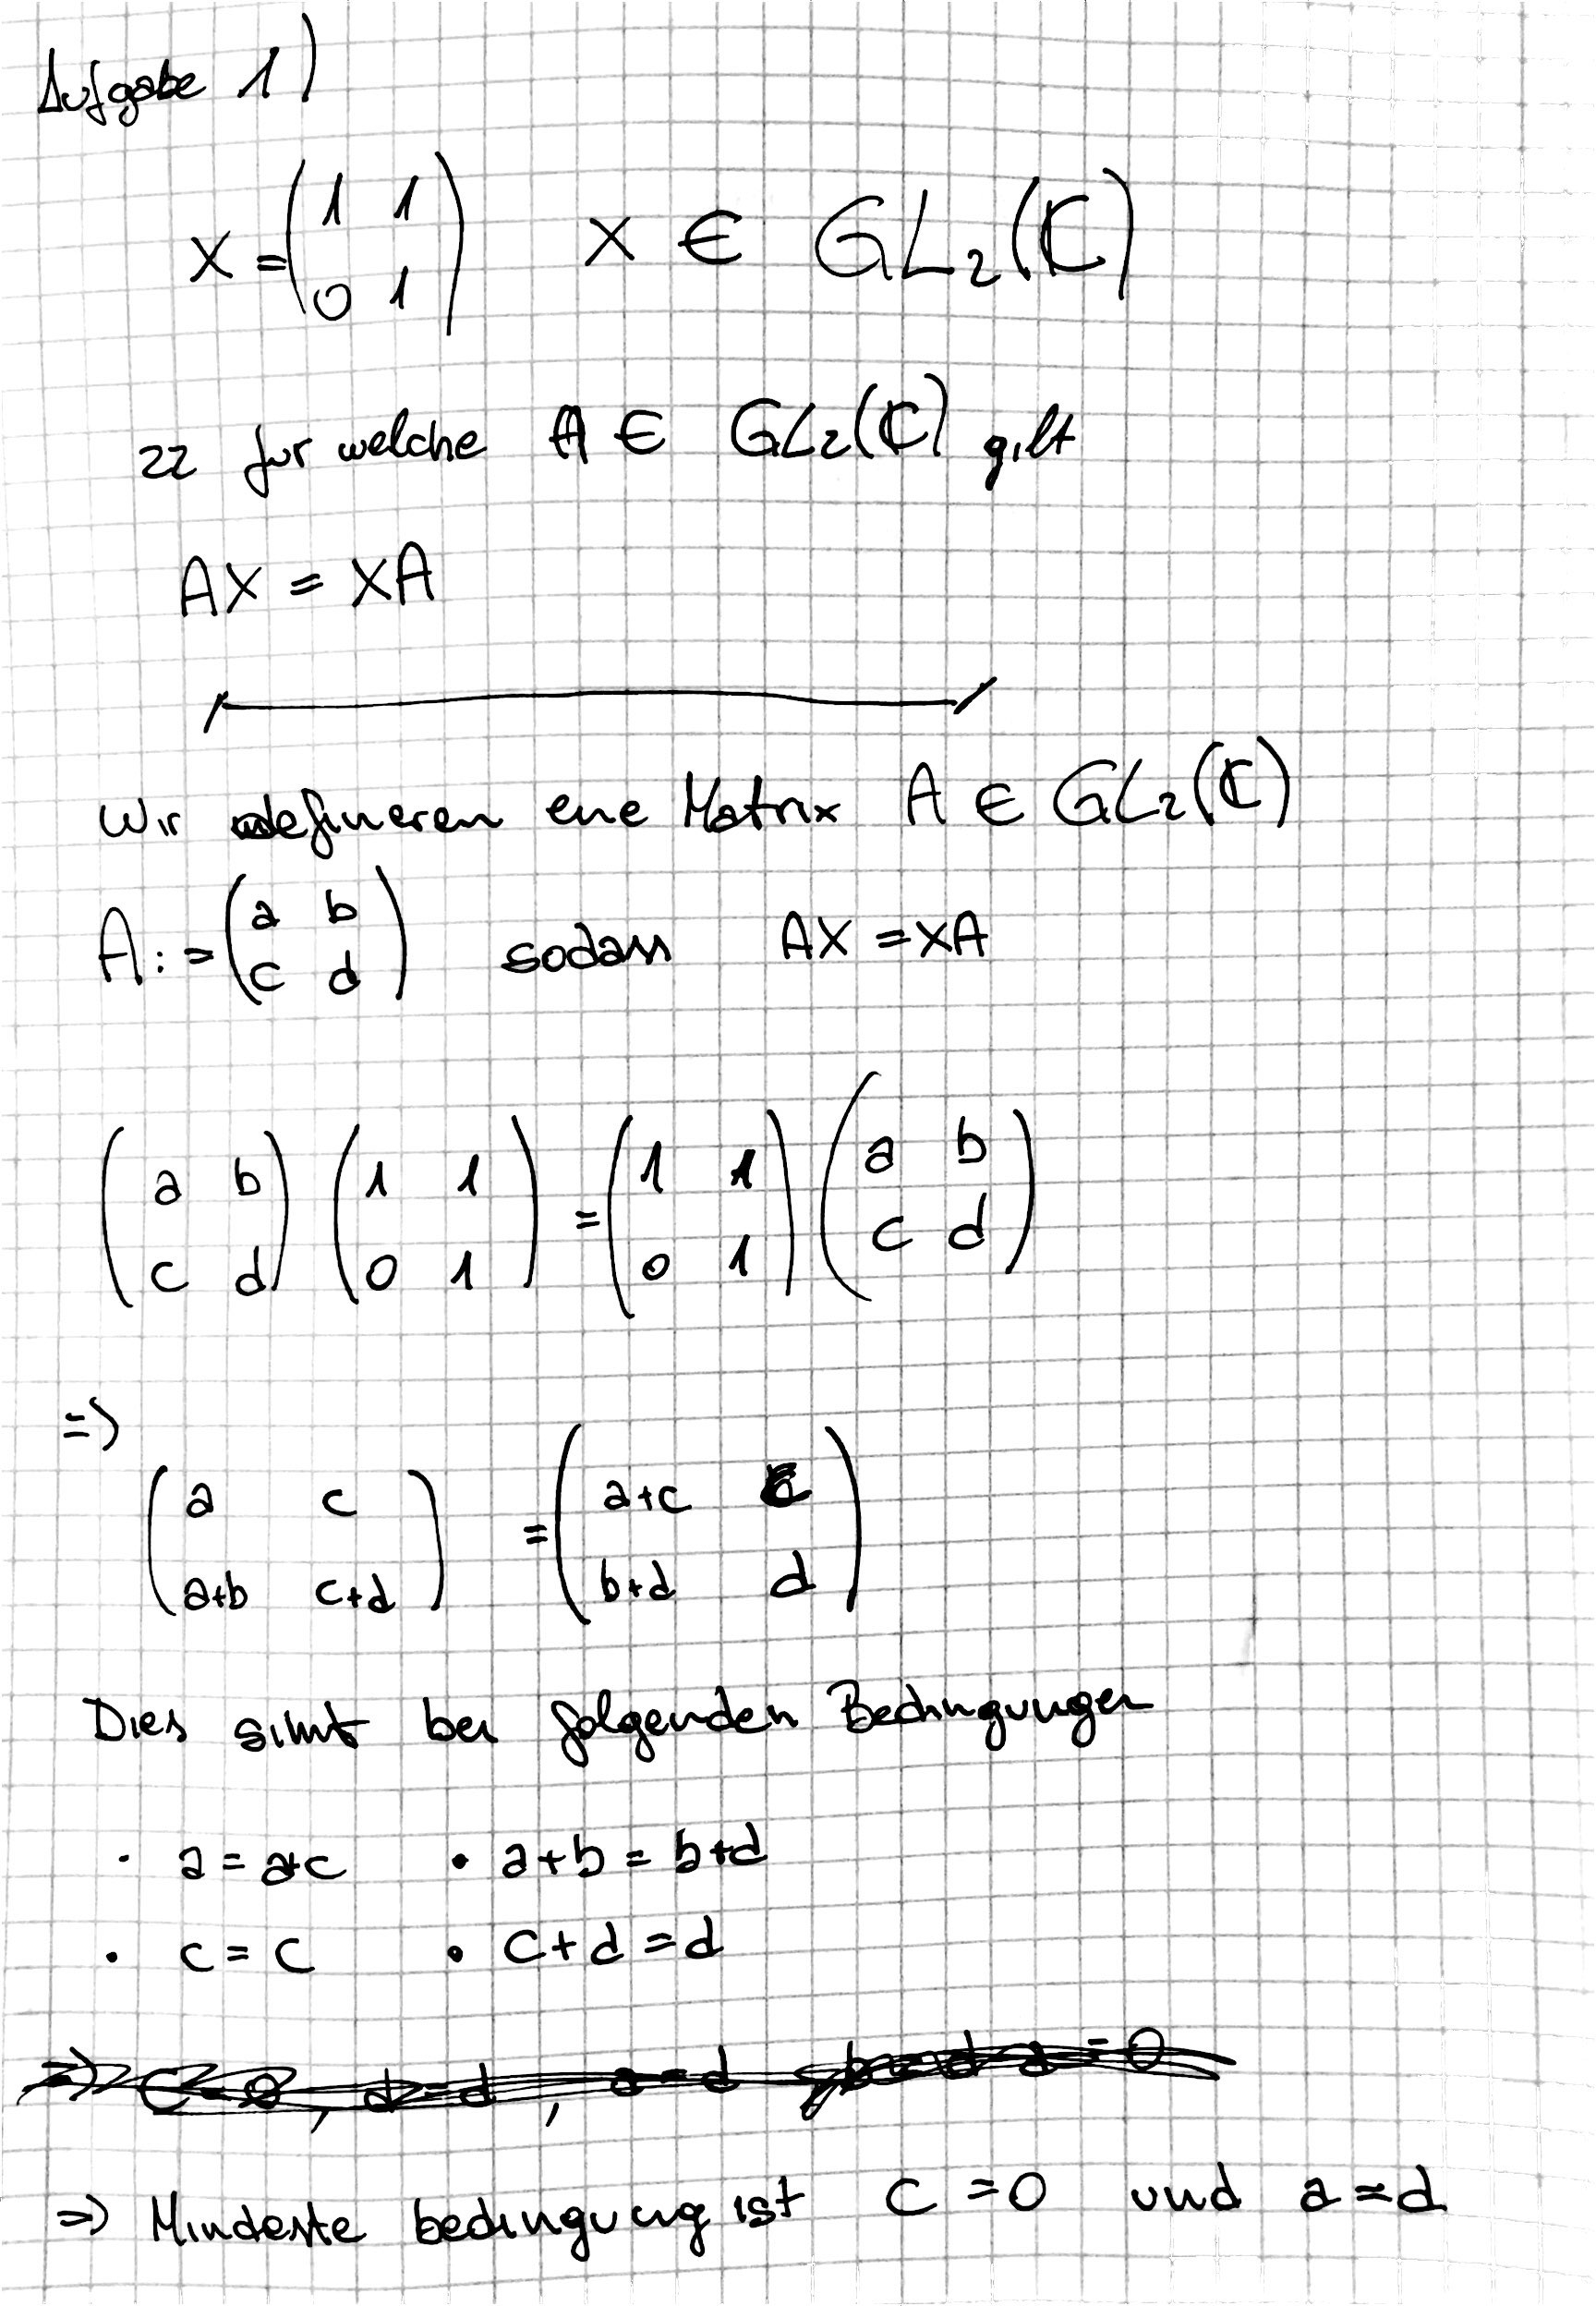
\includegraphics[width=\textwidth]{lat5a_5.jpg} 
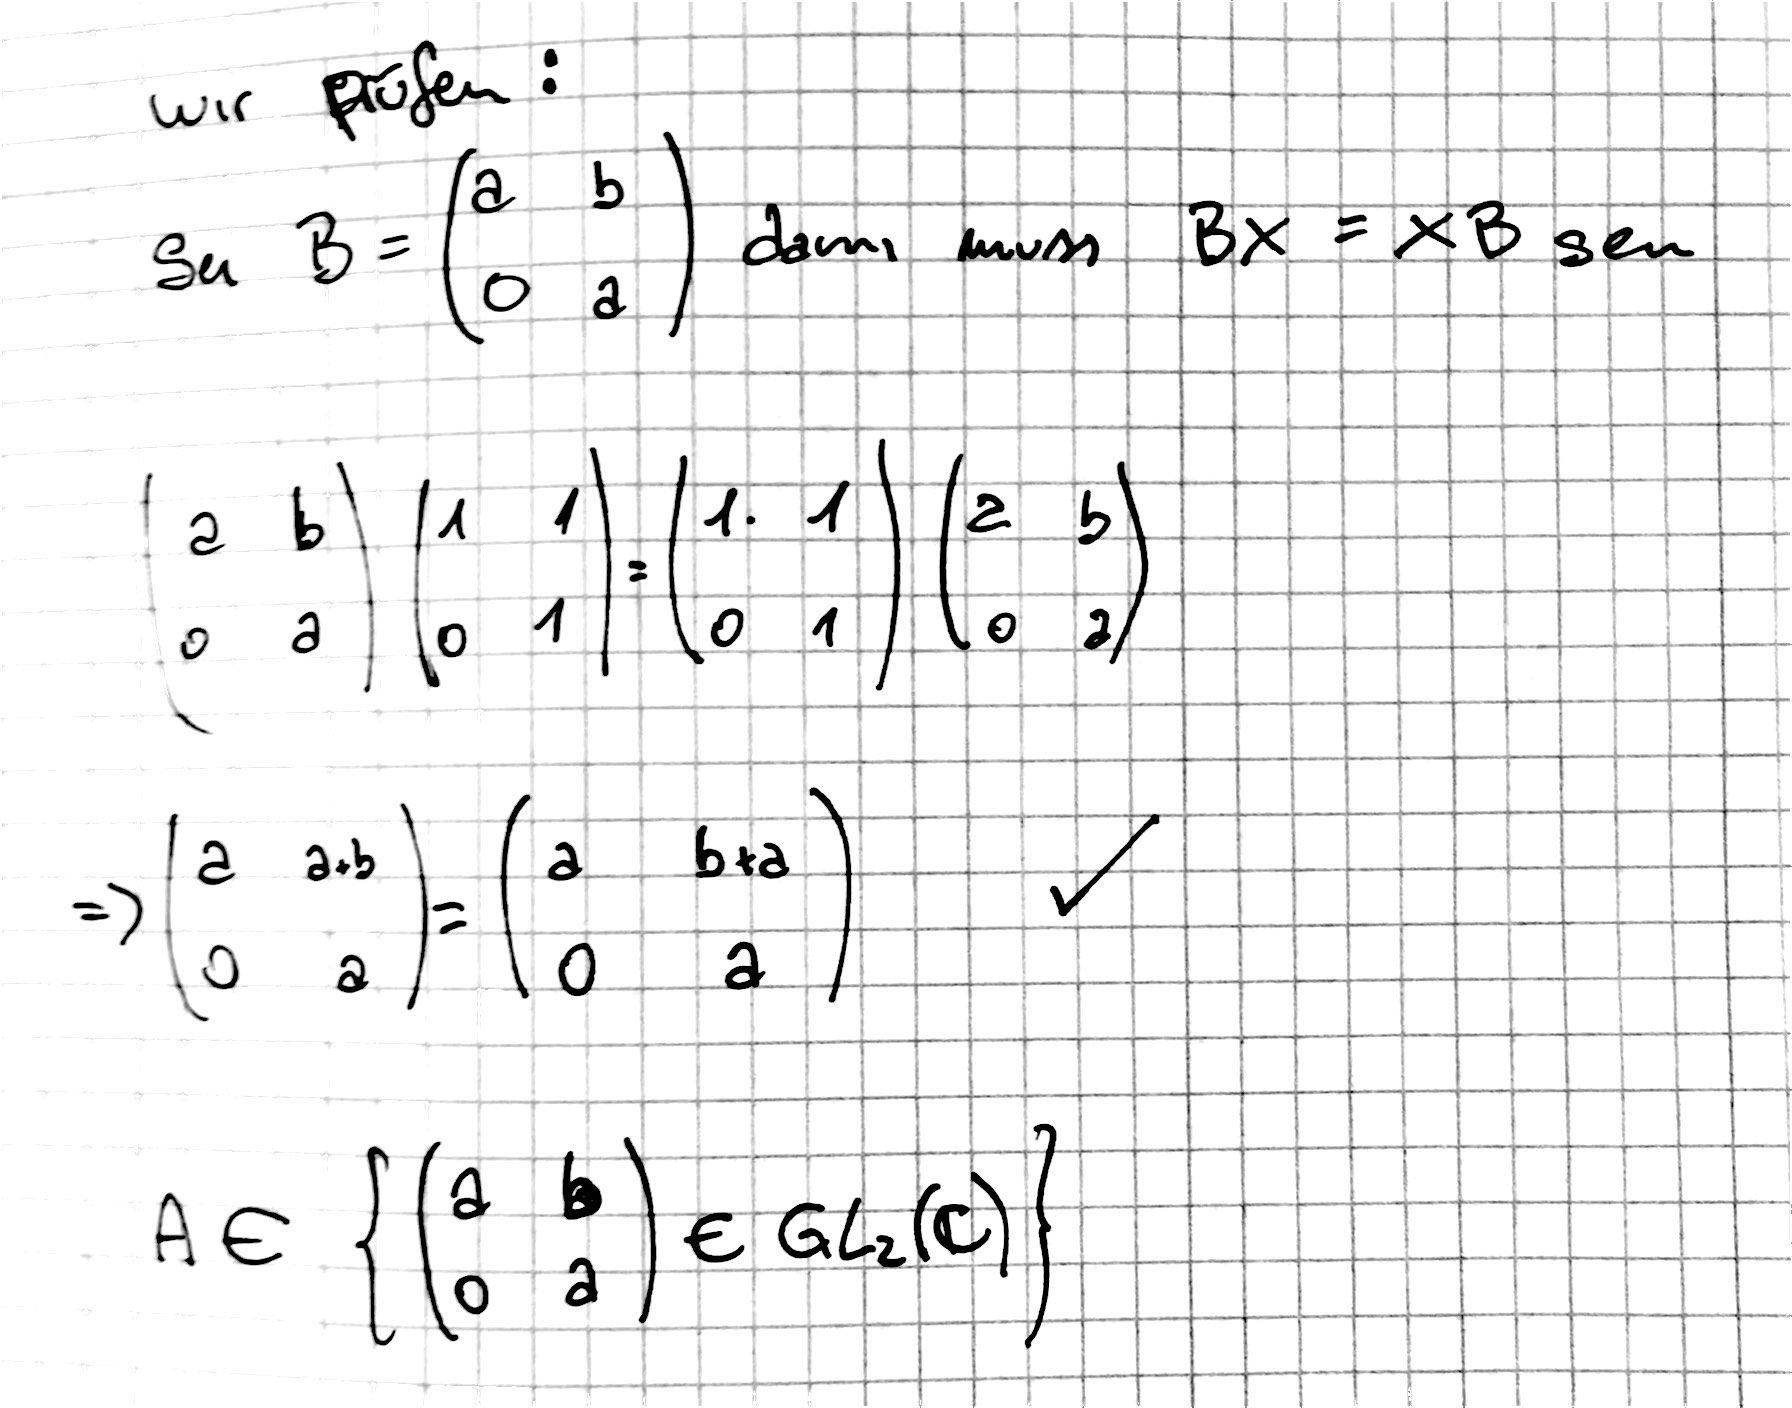
\includegraphics[width=\textwidth]{lat5a_6.jpg} 


\newpage
\section{Aufgabe 2}
\subsection{Nützliche Beweise}
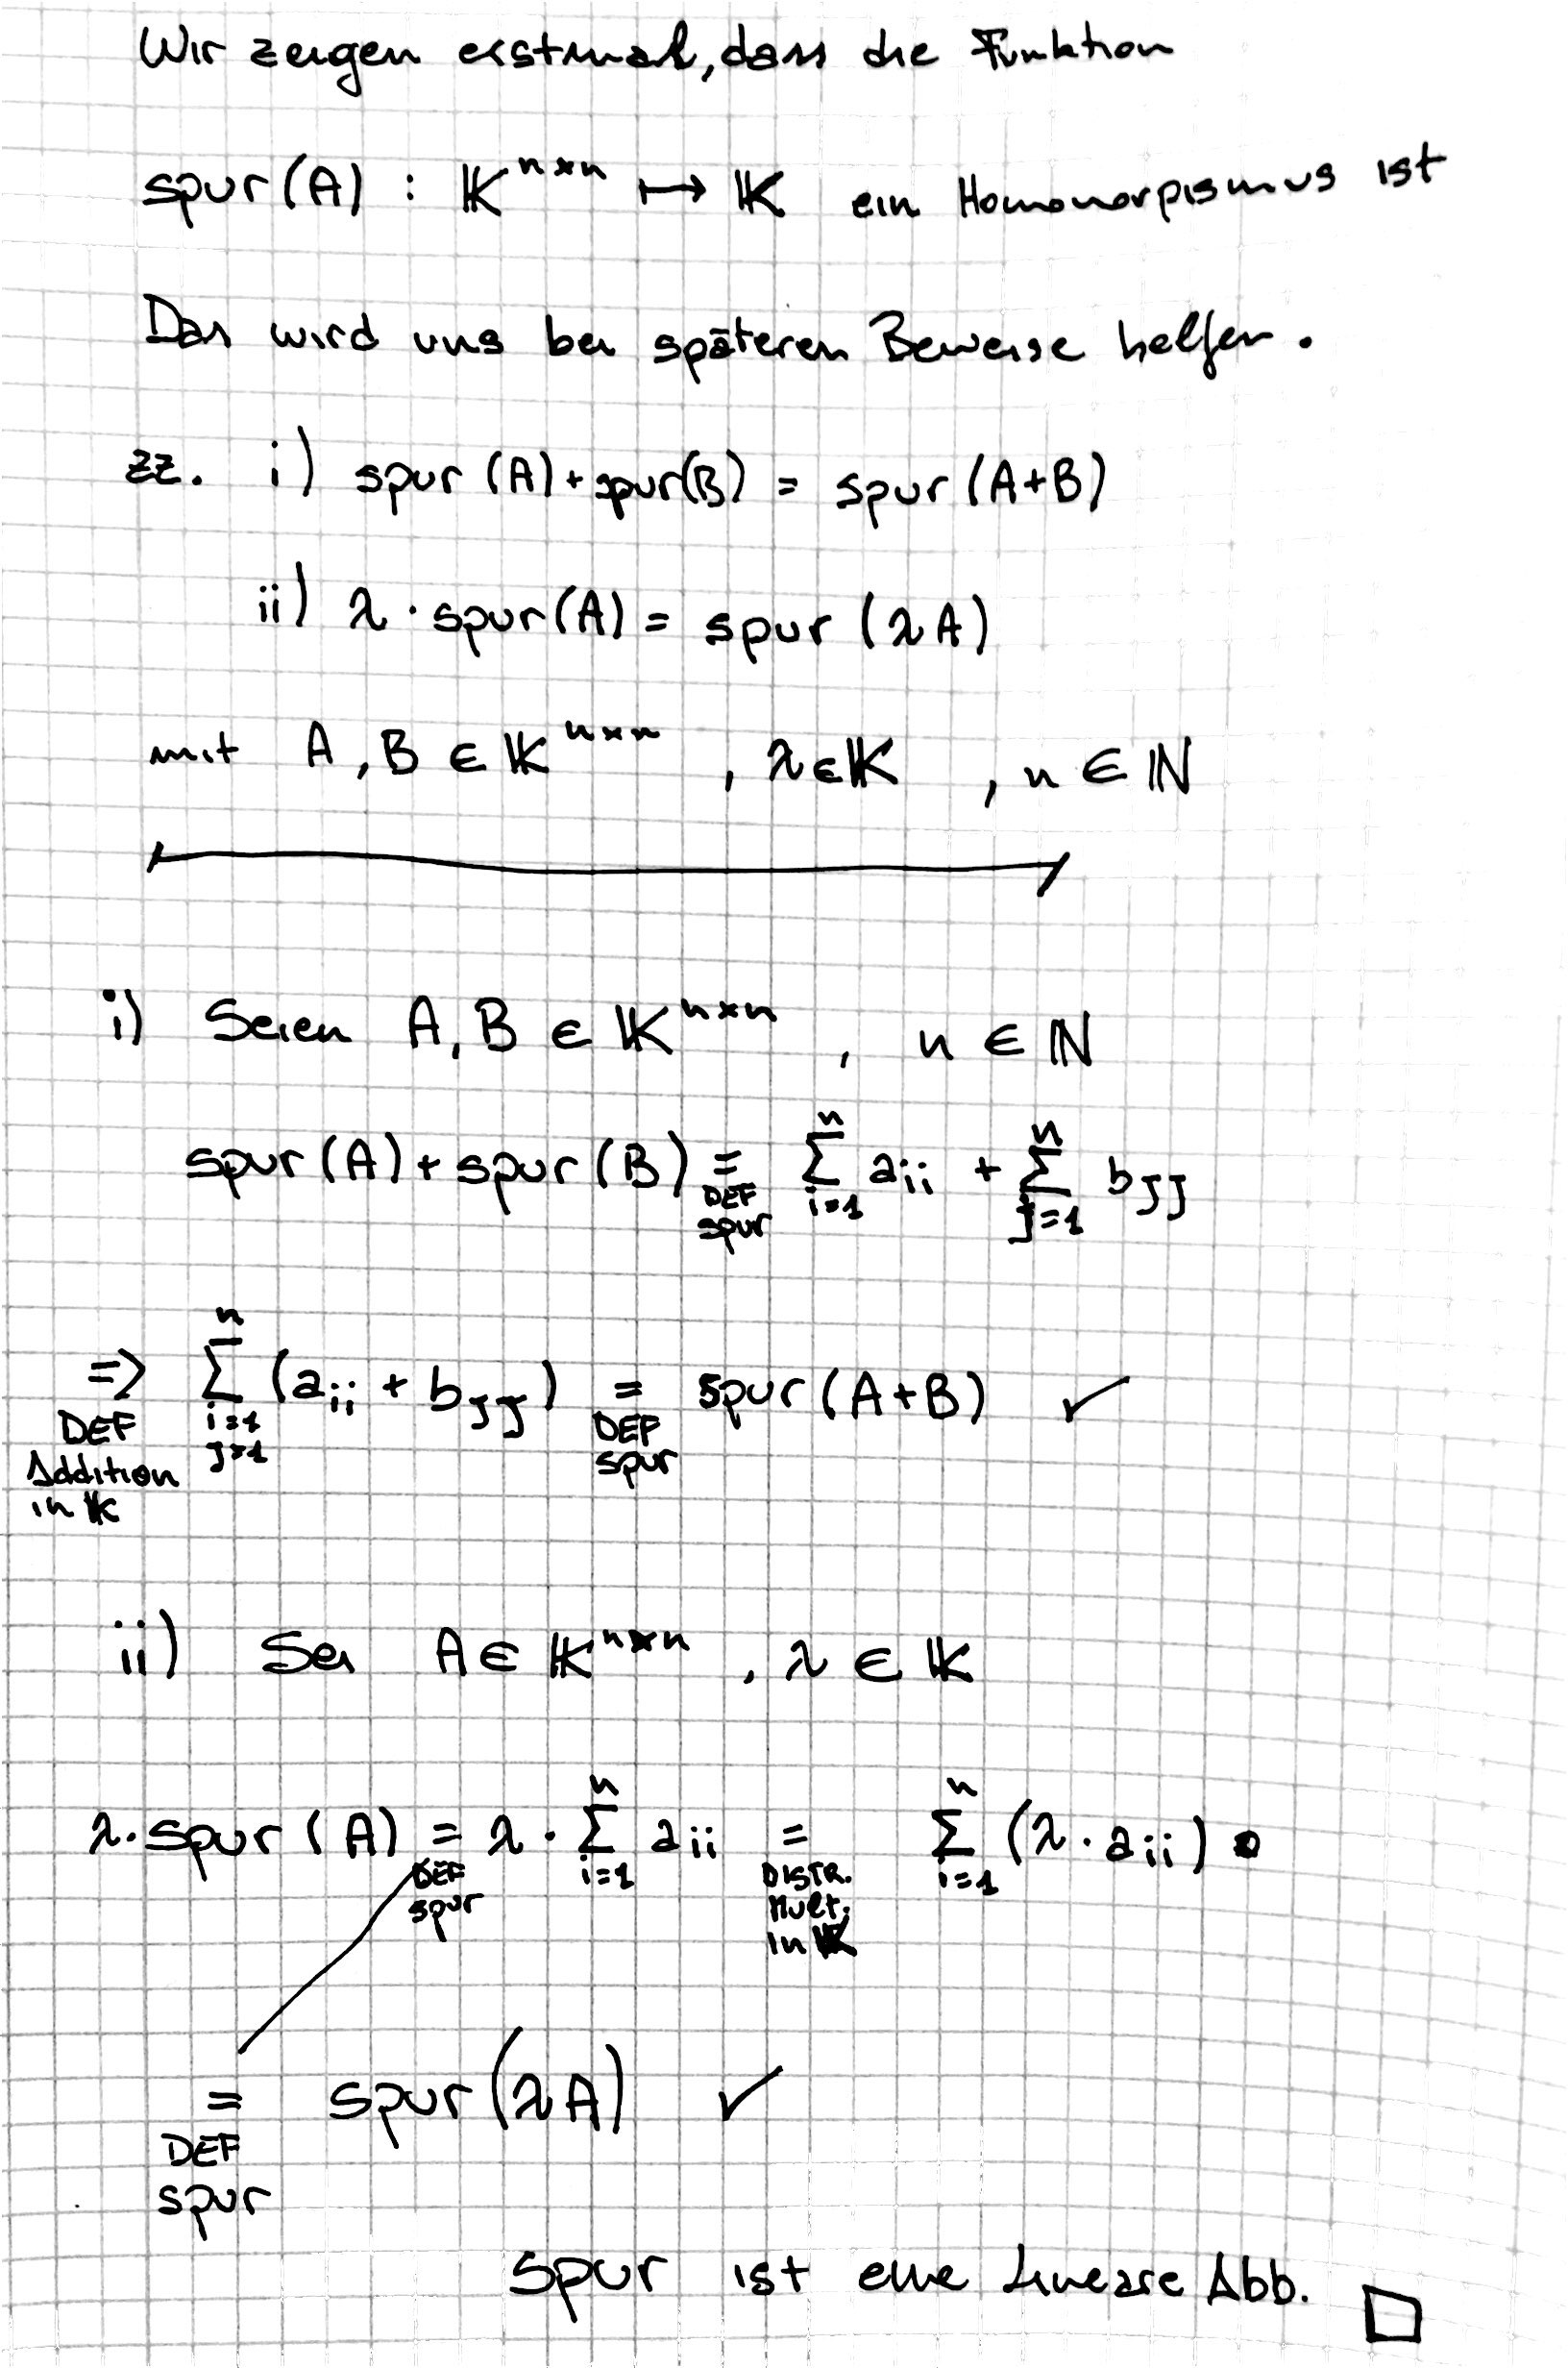
\includegraphics[width=\textwidth]{lat5a_1.jpg} 
\subsection{i}
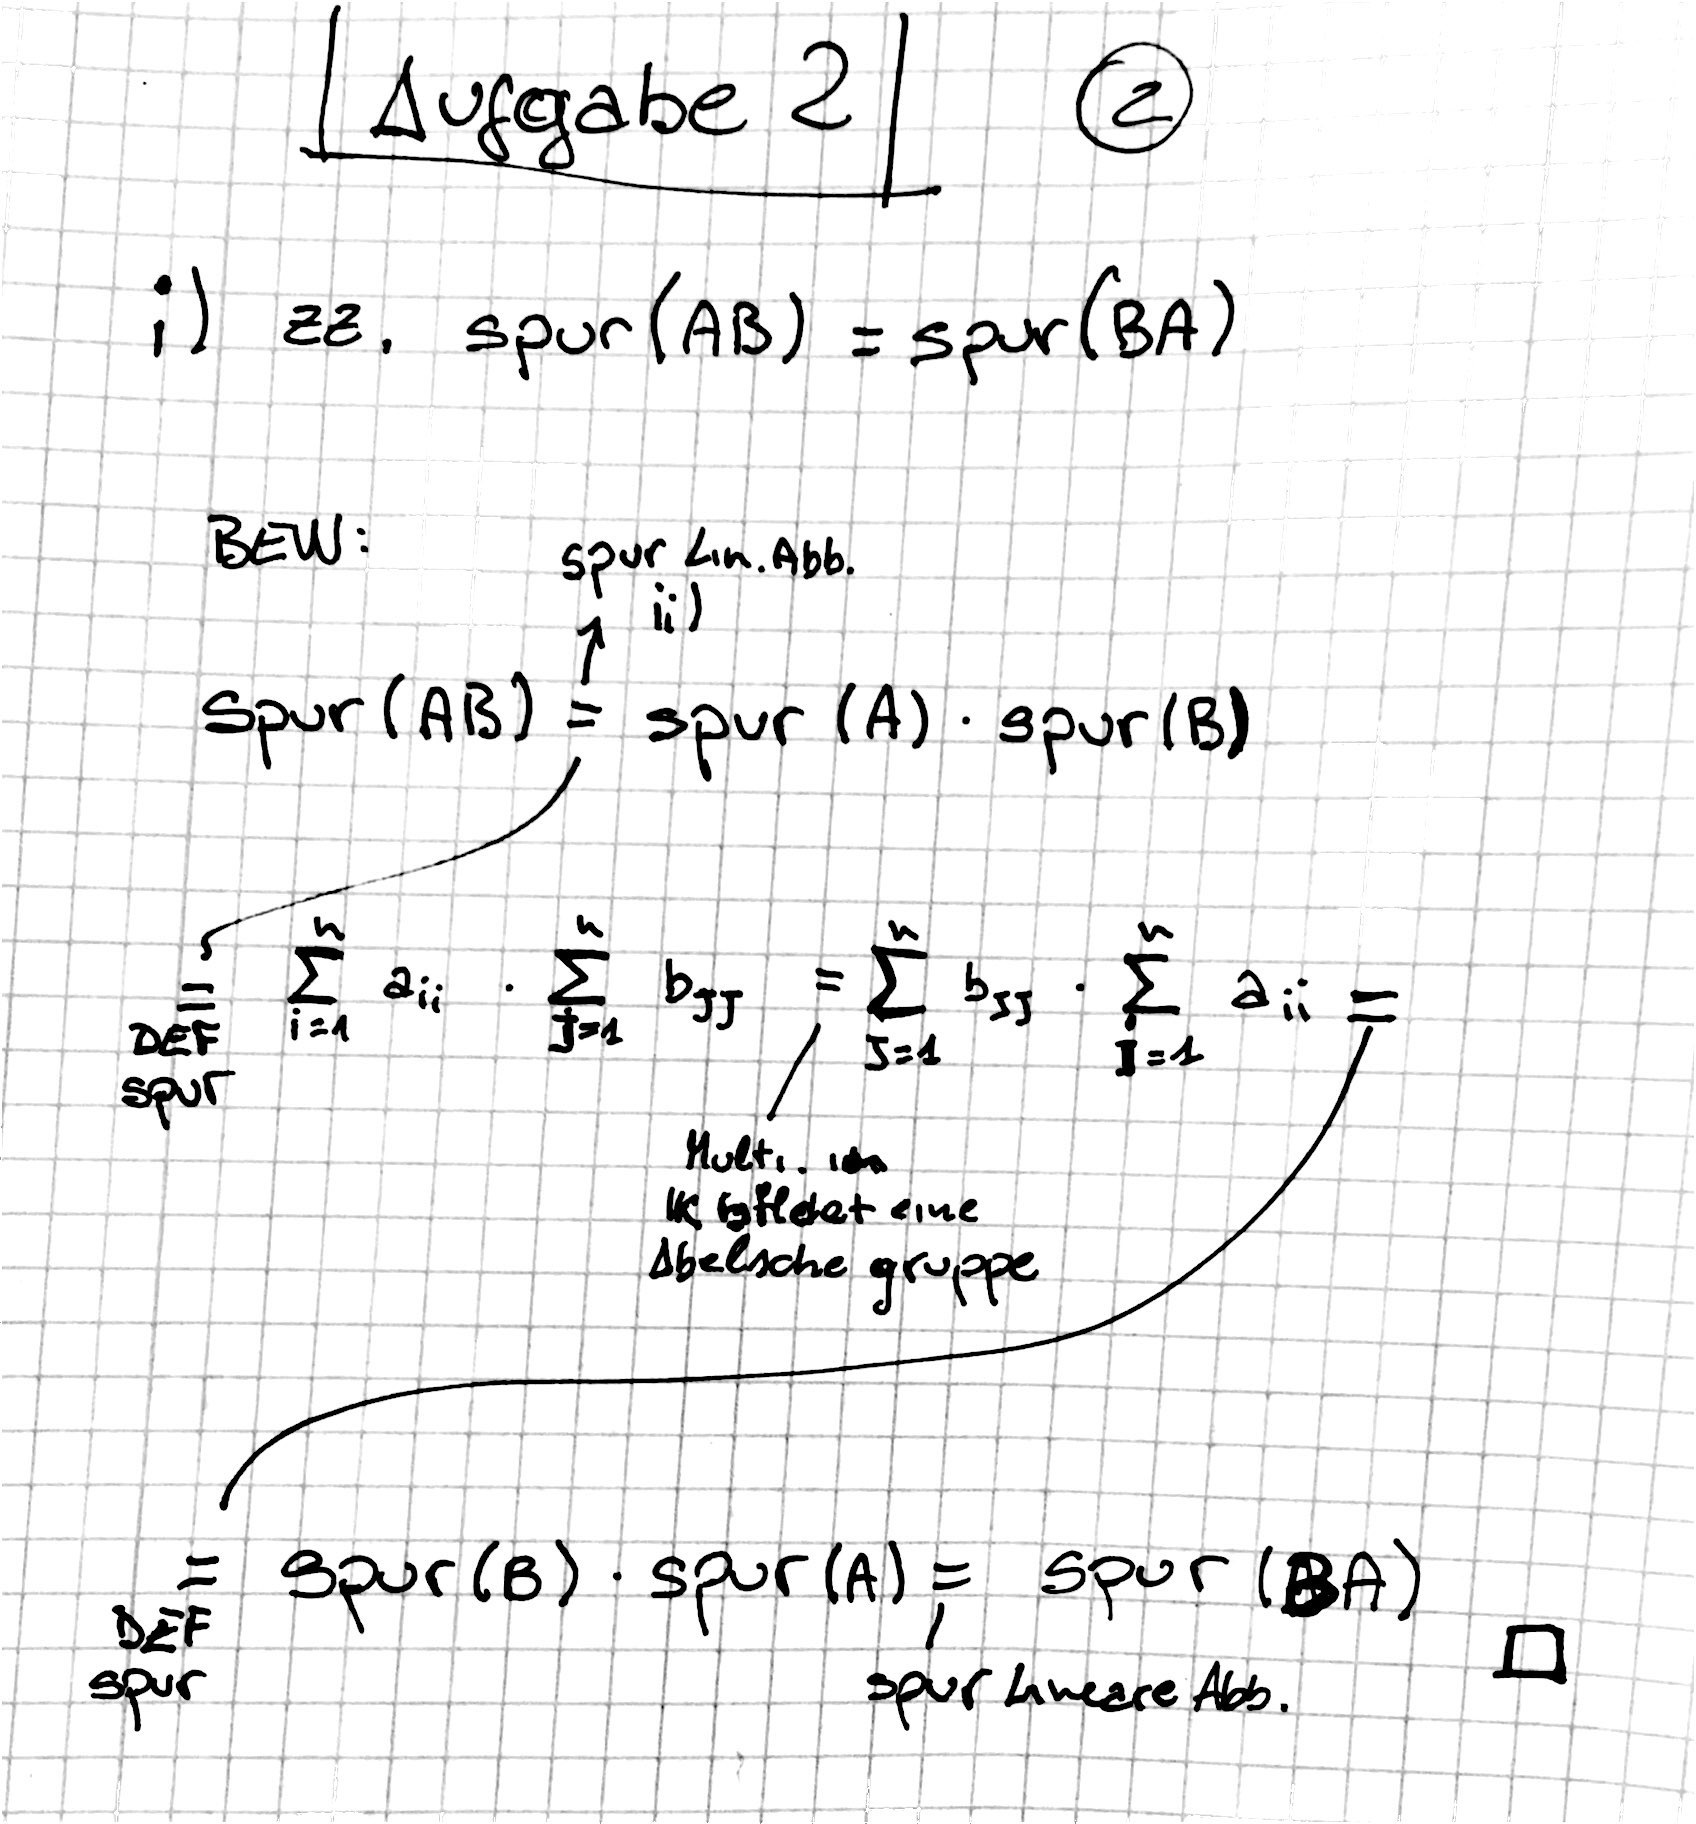
\includegraphics[width=\textwidth]{lat5a_2.jpg} 
\subsection{ii}
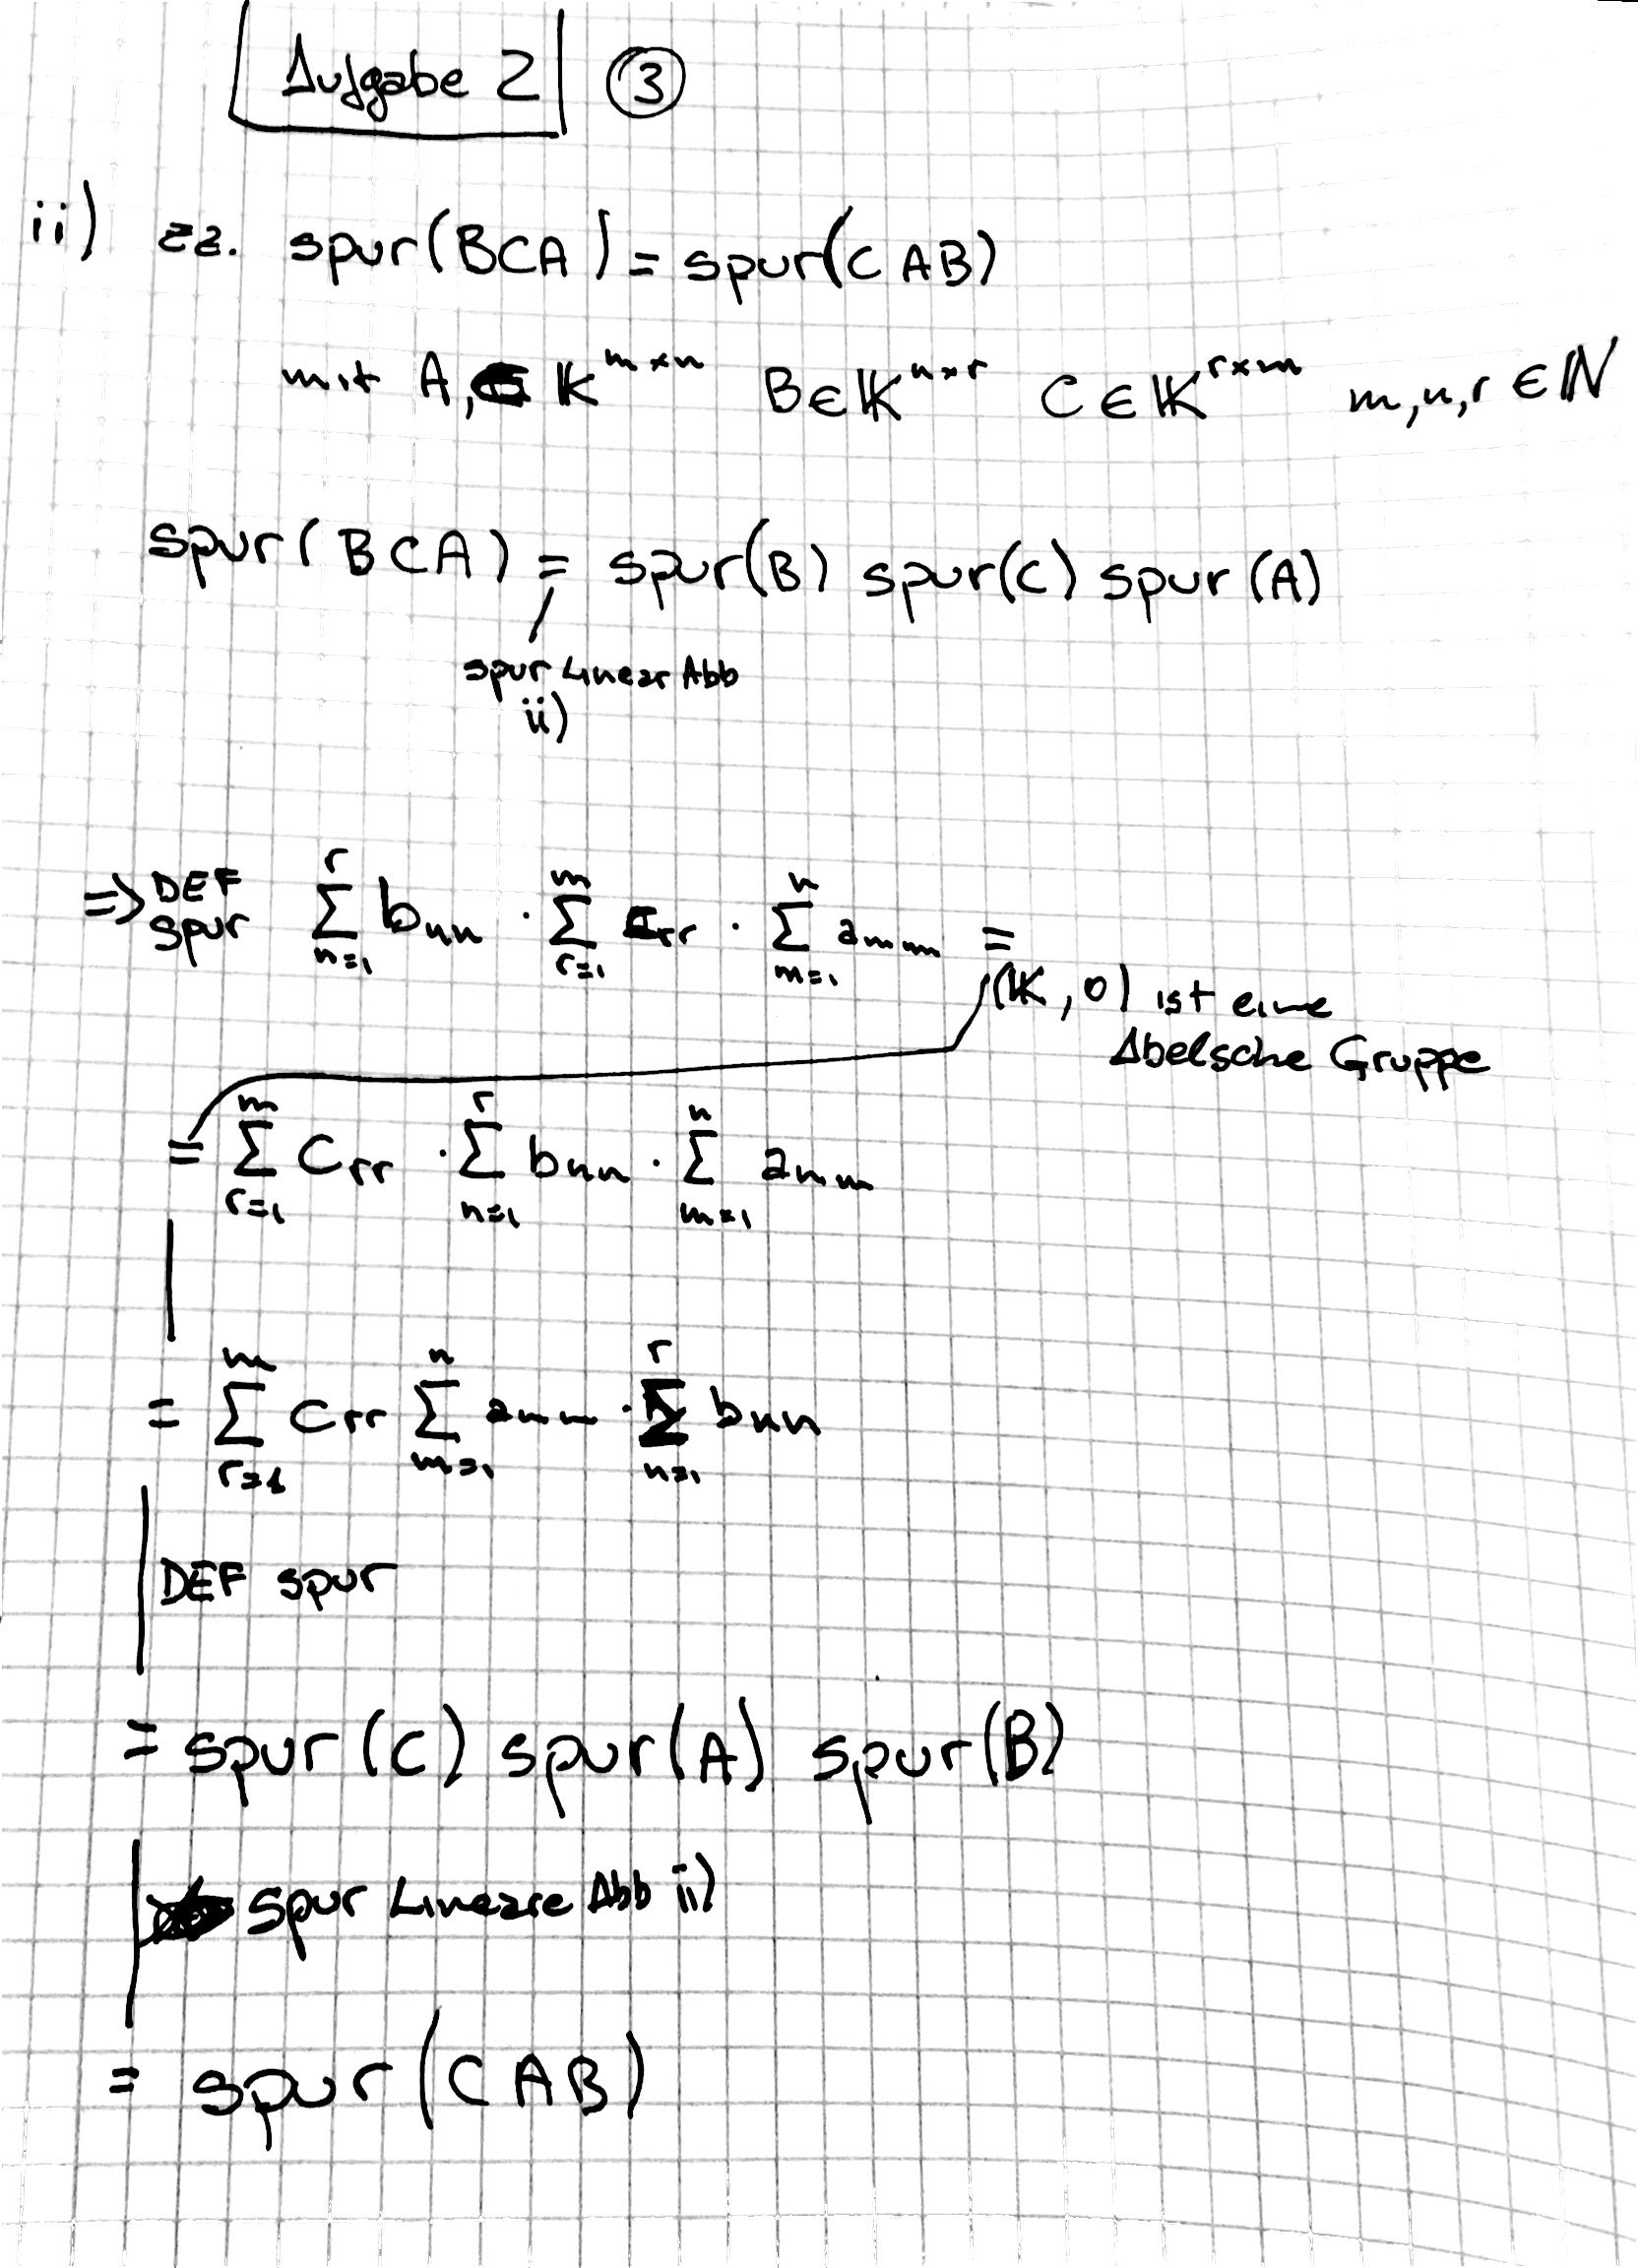
\includegraphics[width=\textwidth]{lat5a_3.jpg} 
\subsection{iii}
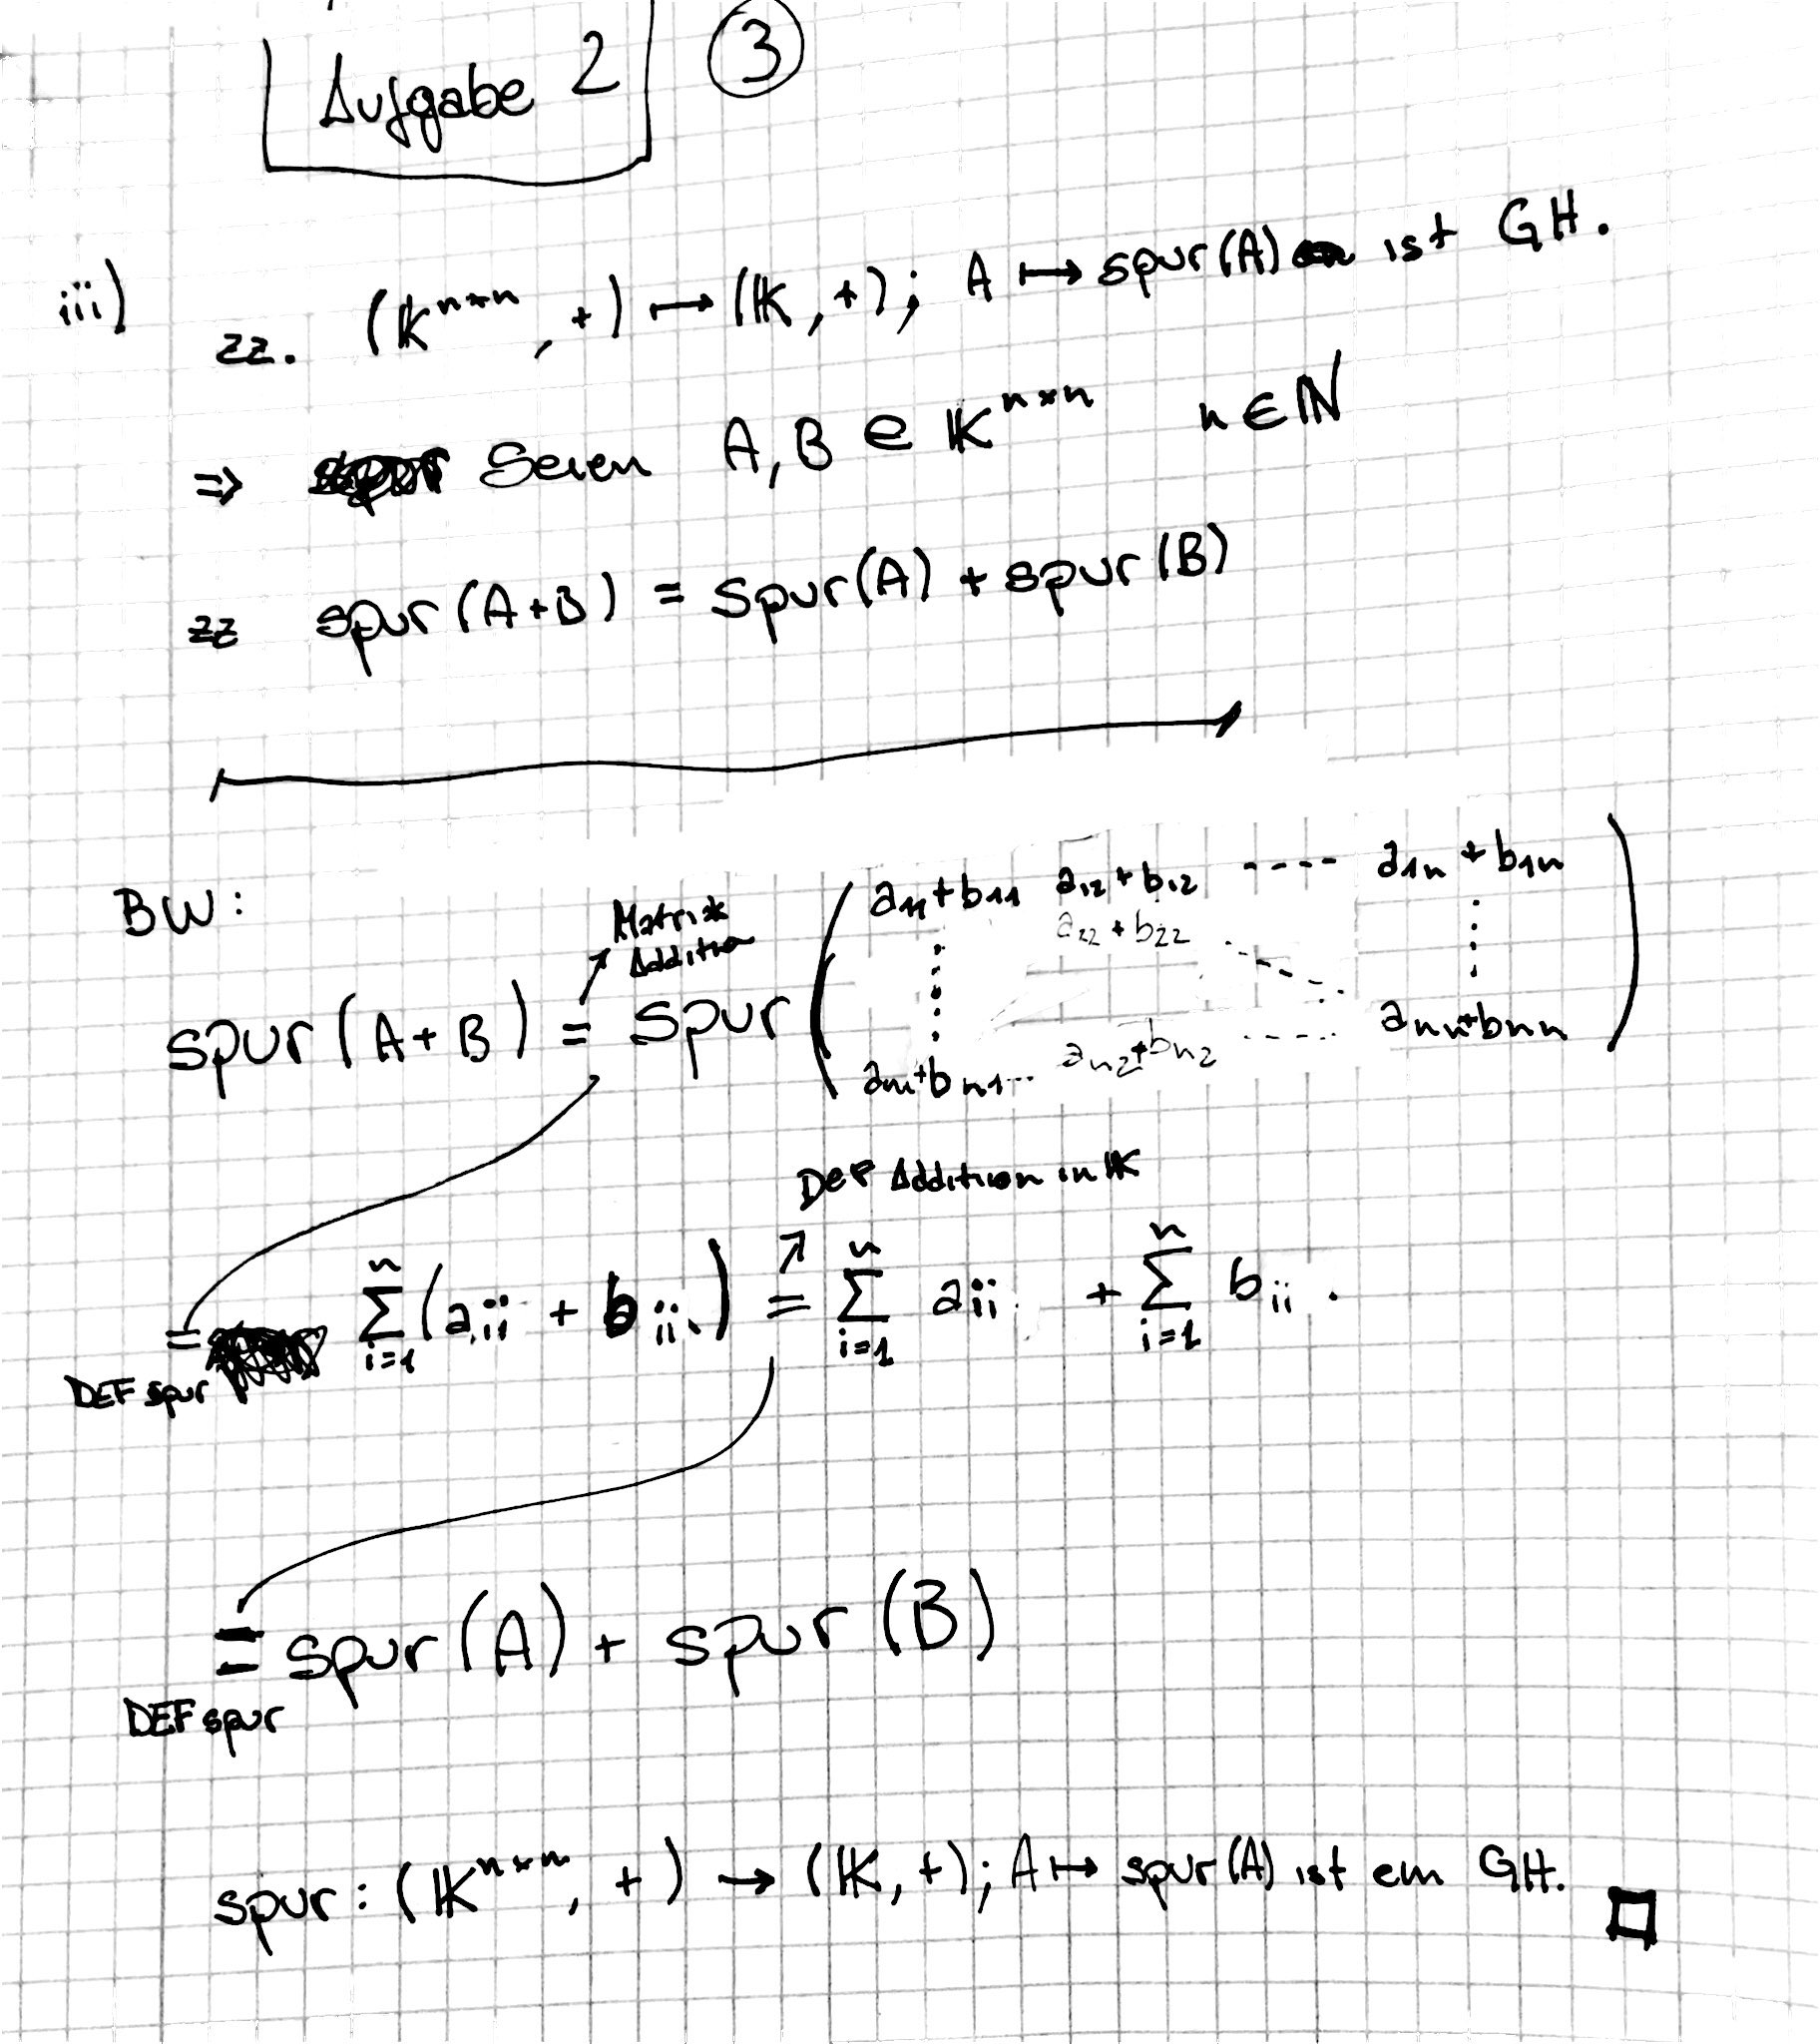
\includegraphics[width=\textwidth]{lat5a_4.jpg} 


\newpage
\section{Aufgabe 3}
\subsection{i}
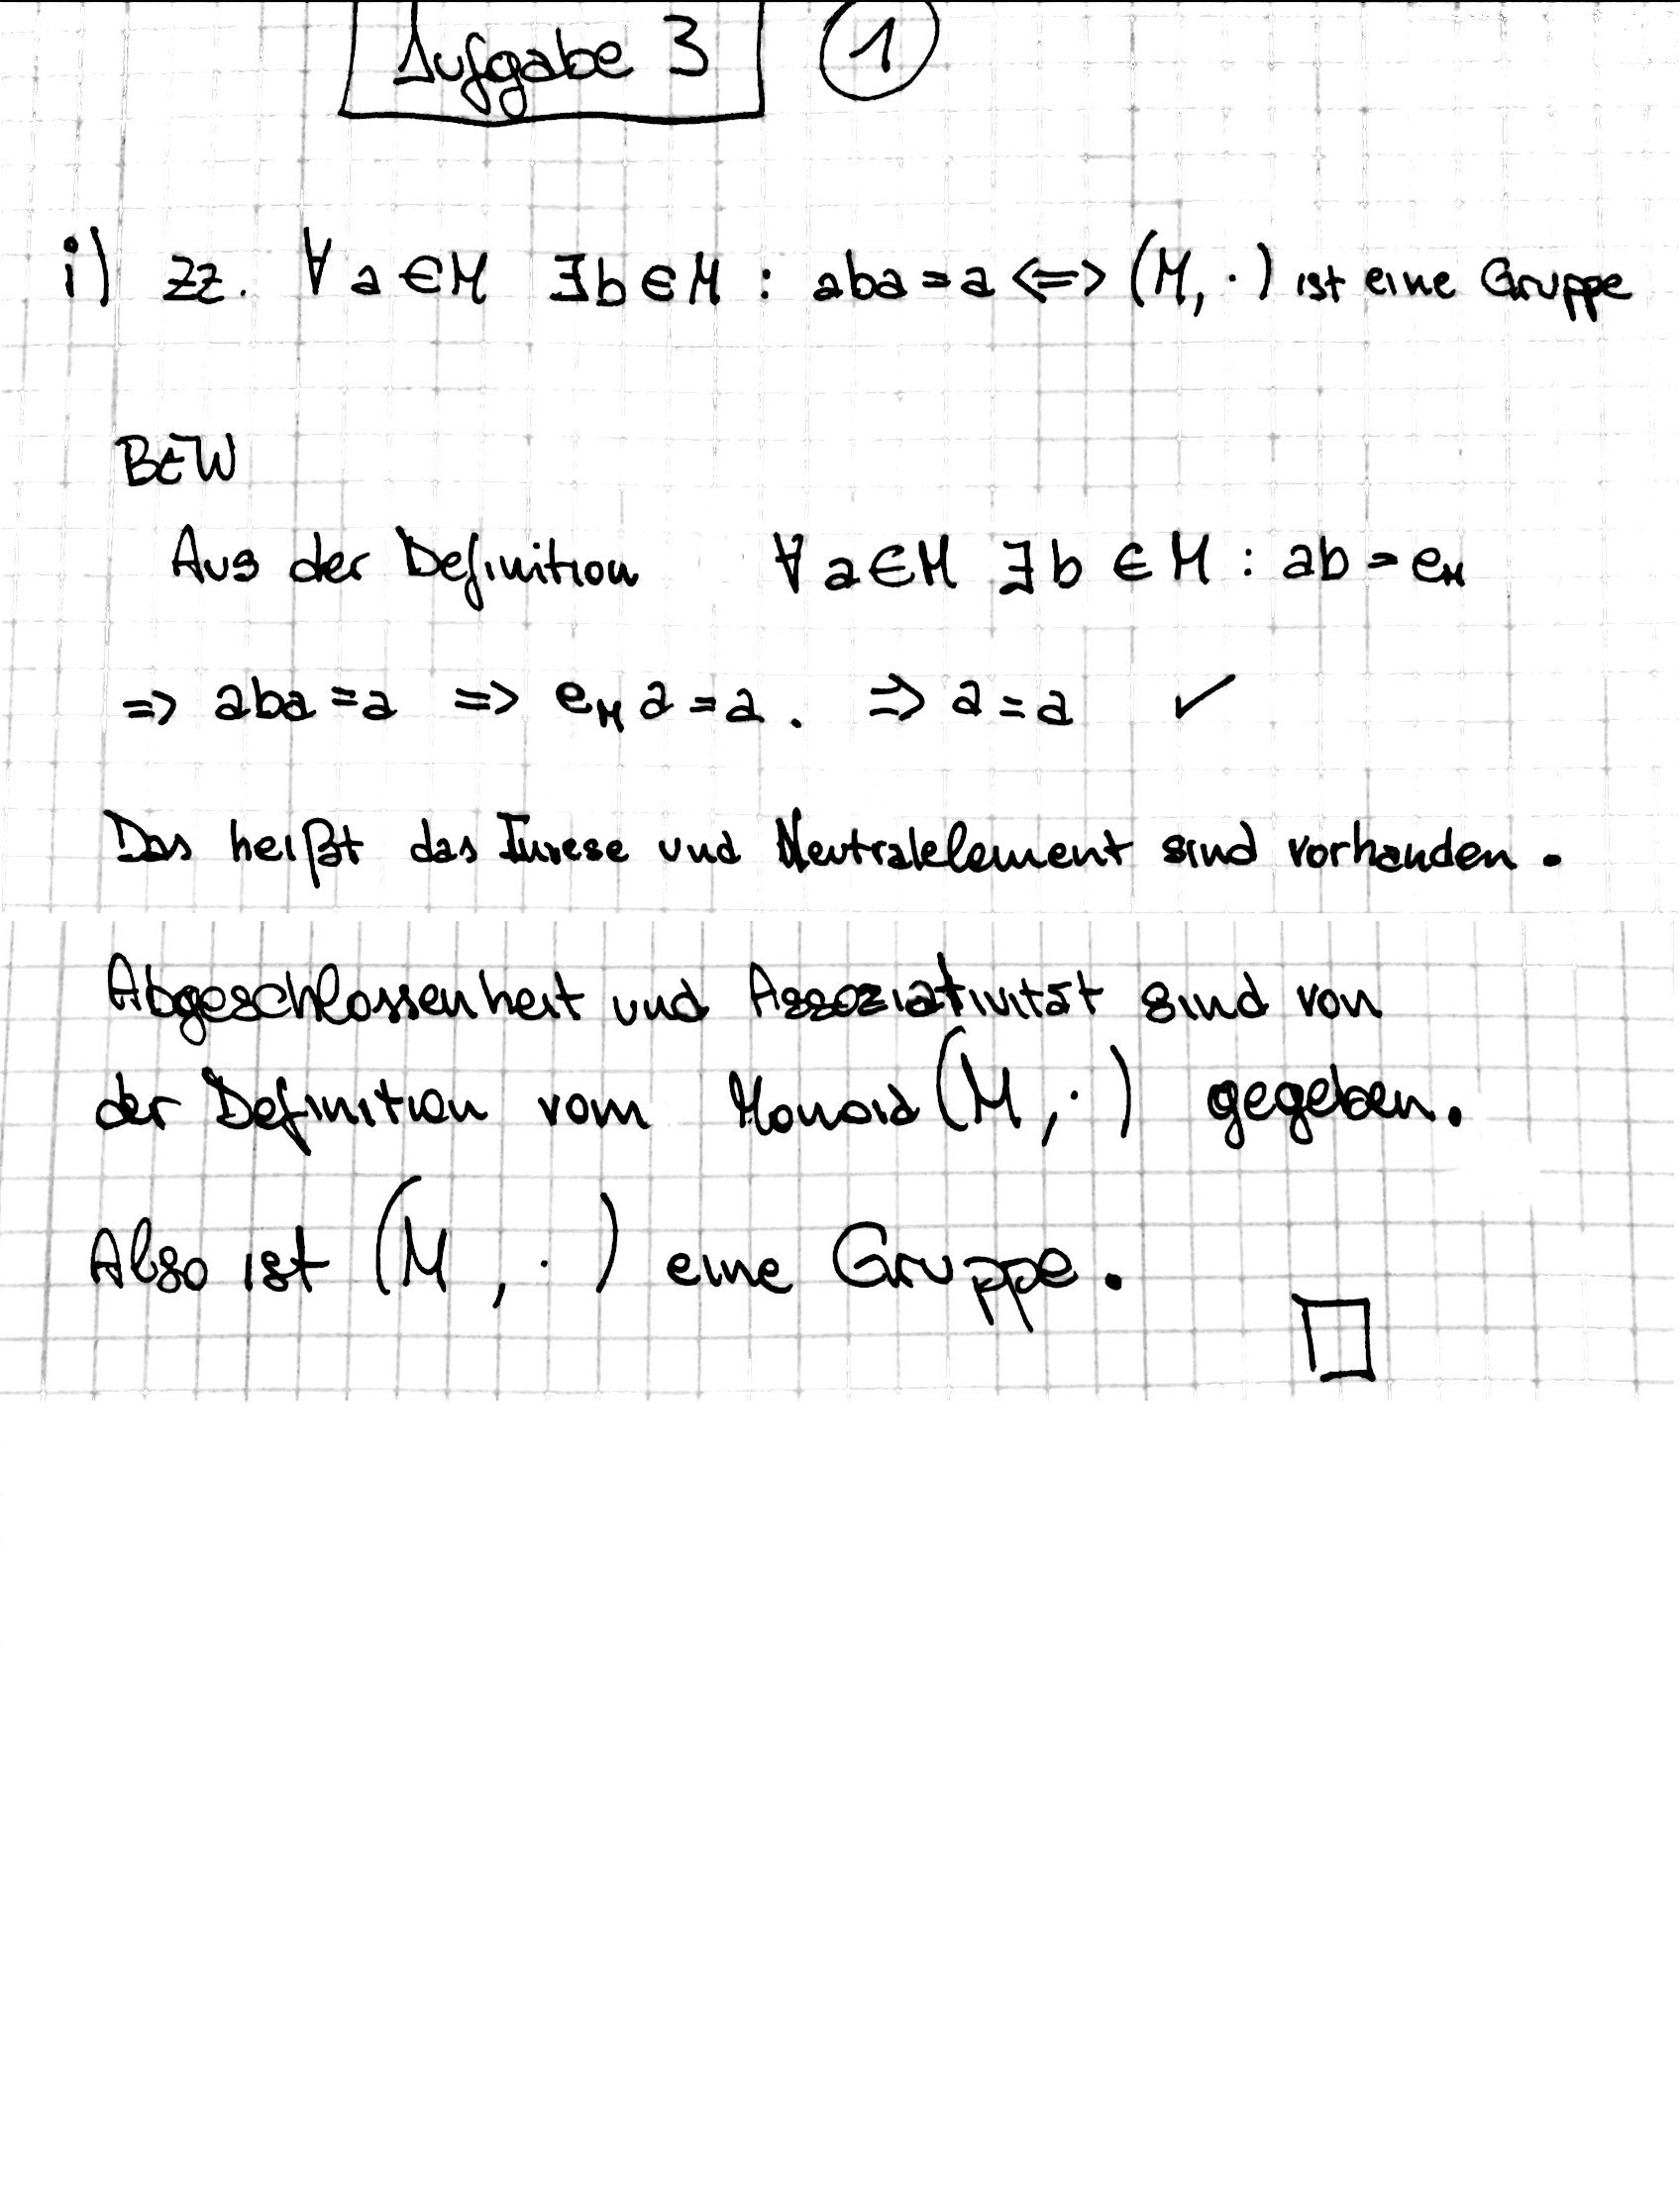
\includegraphics[width=\textwidth]{lat5b_10.jpg} 
\subsection{ii}
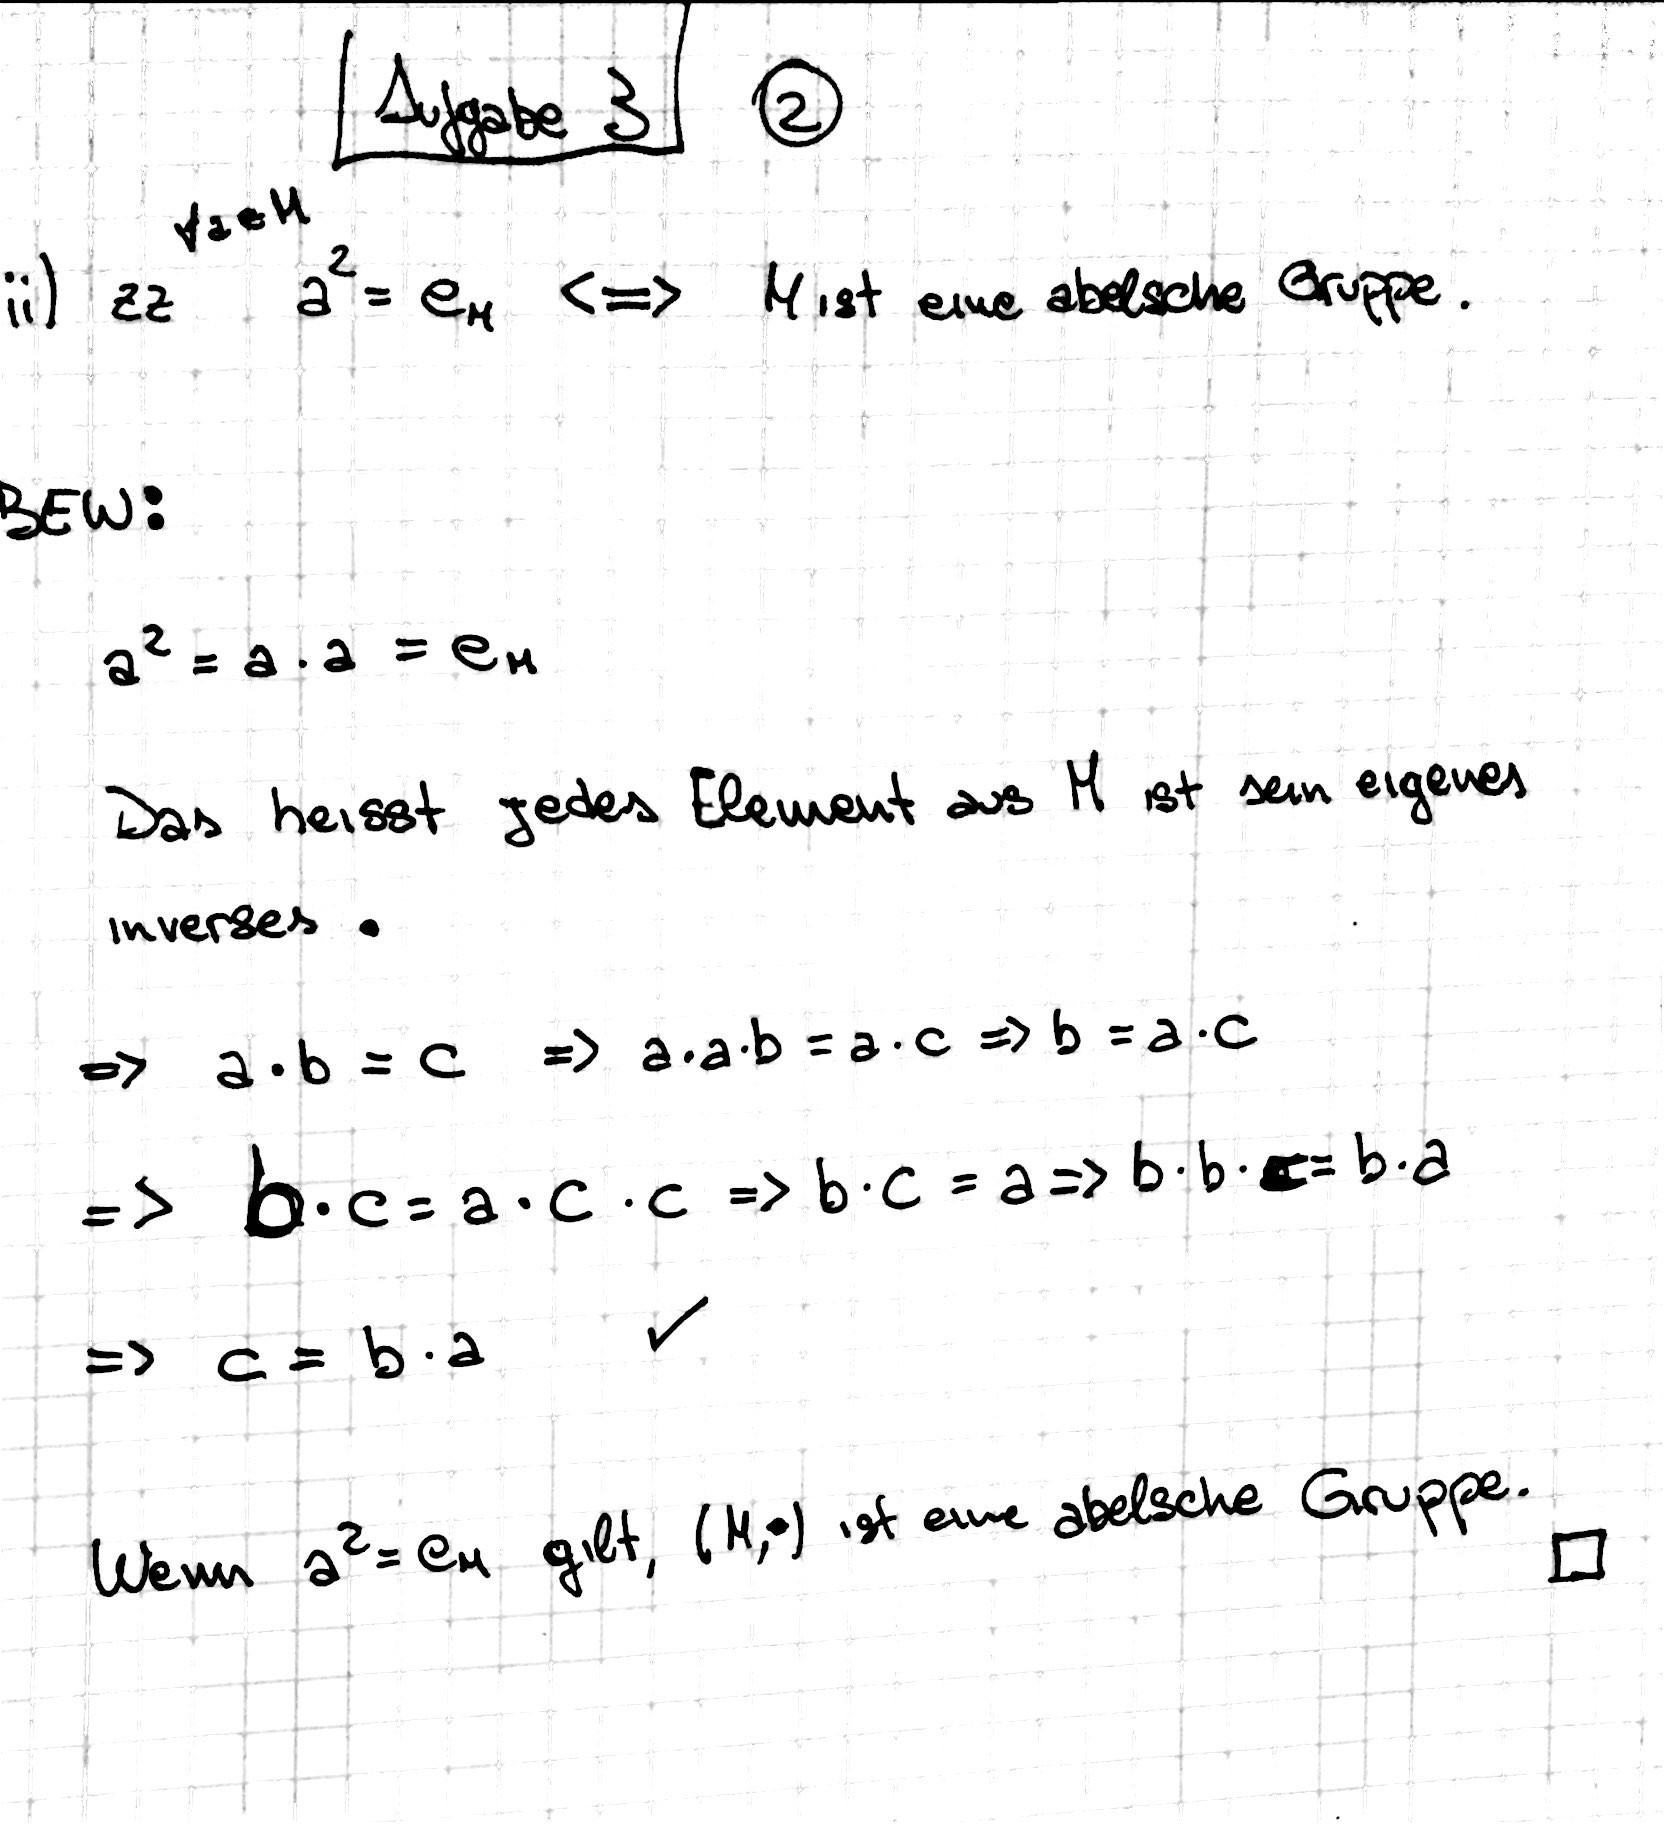
\includegraphics[width=\textwidth]{lat5b_11.jpg} 

\newpage
\section{Aufgabe 4}
\subsection{i}
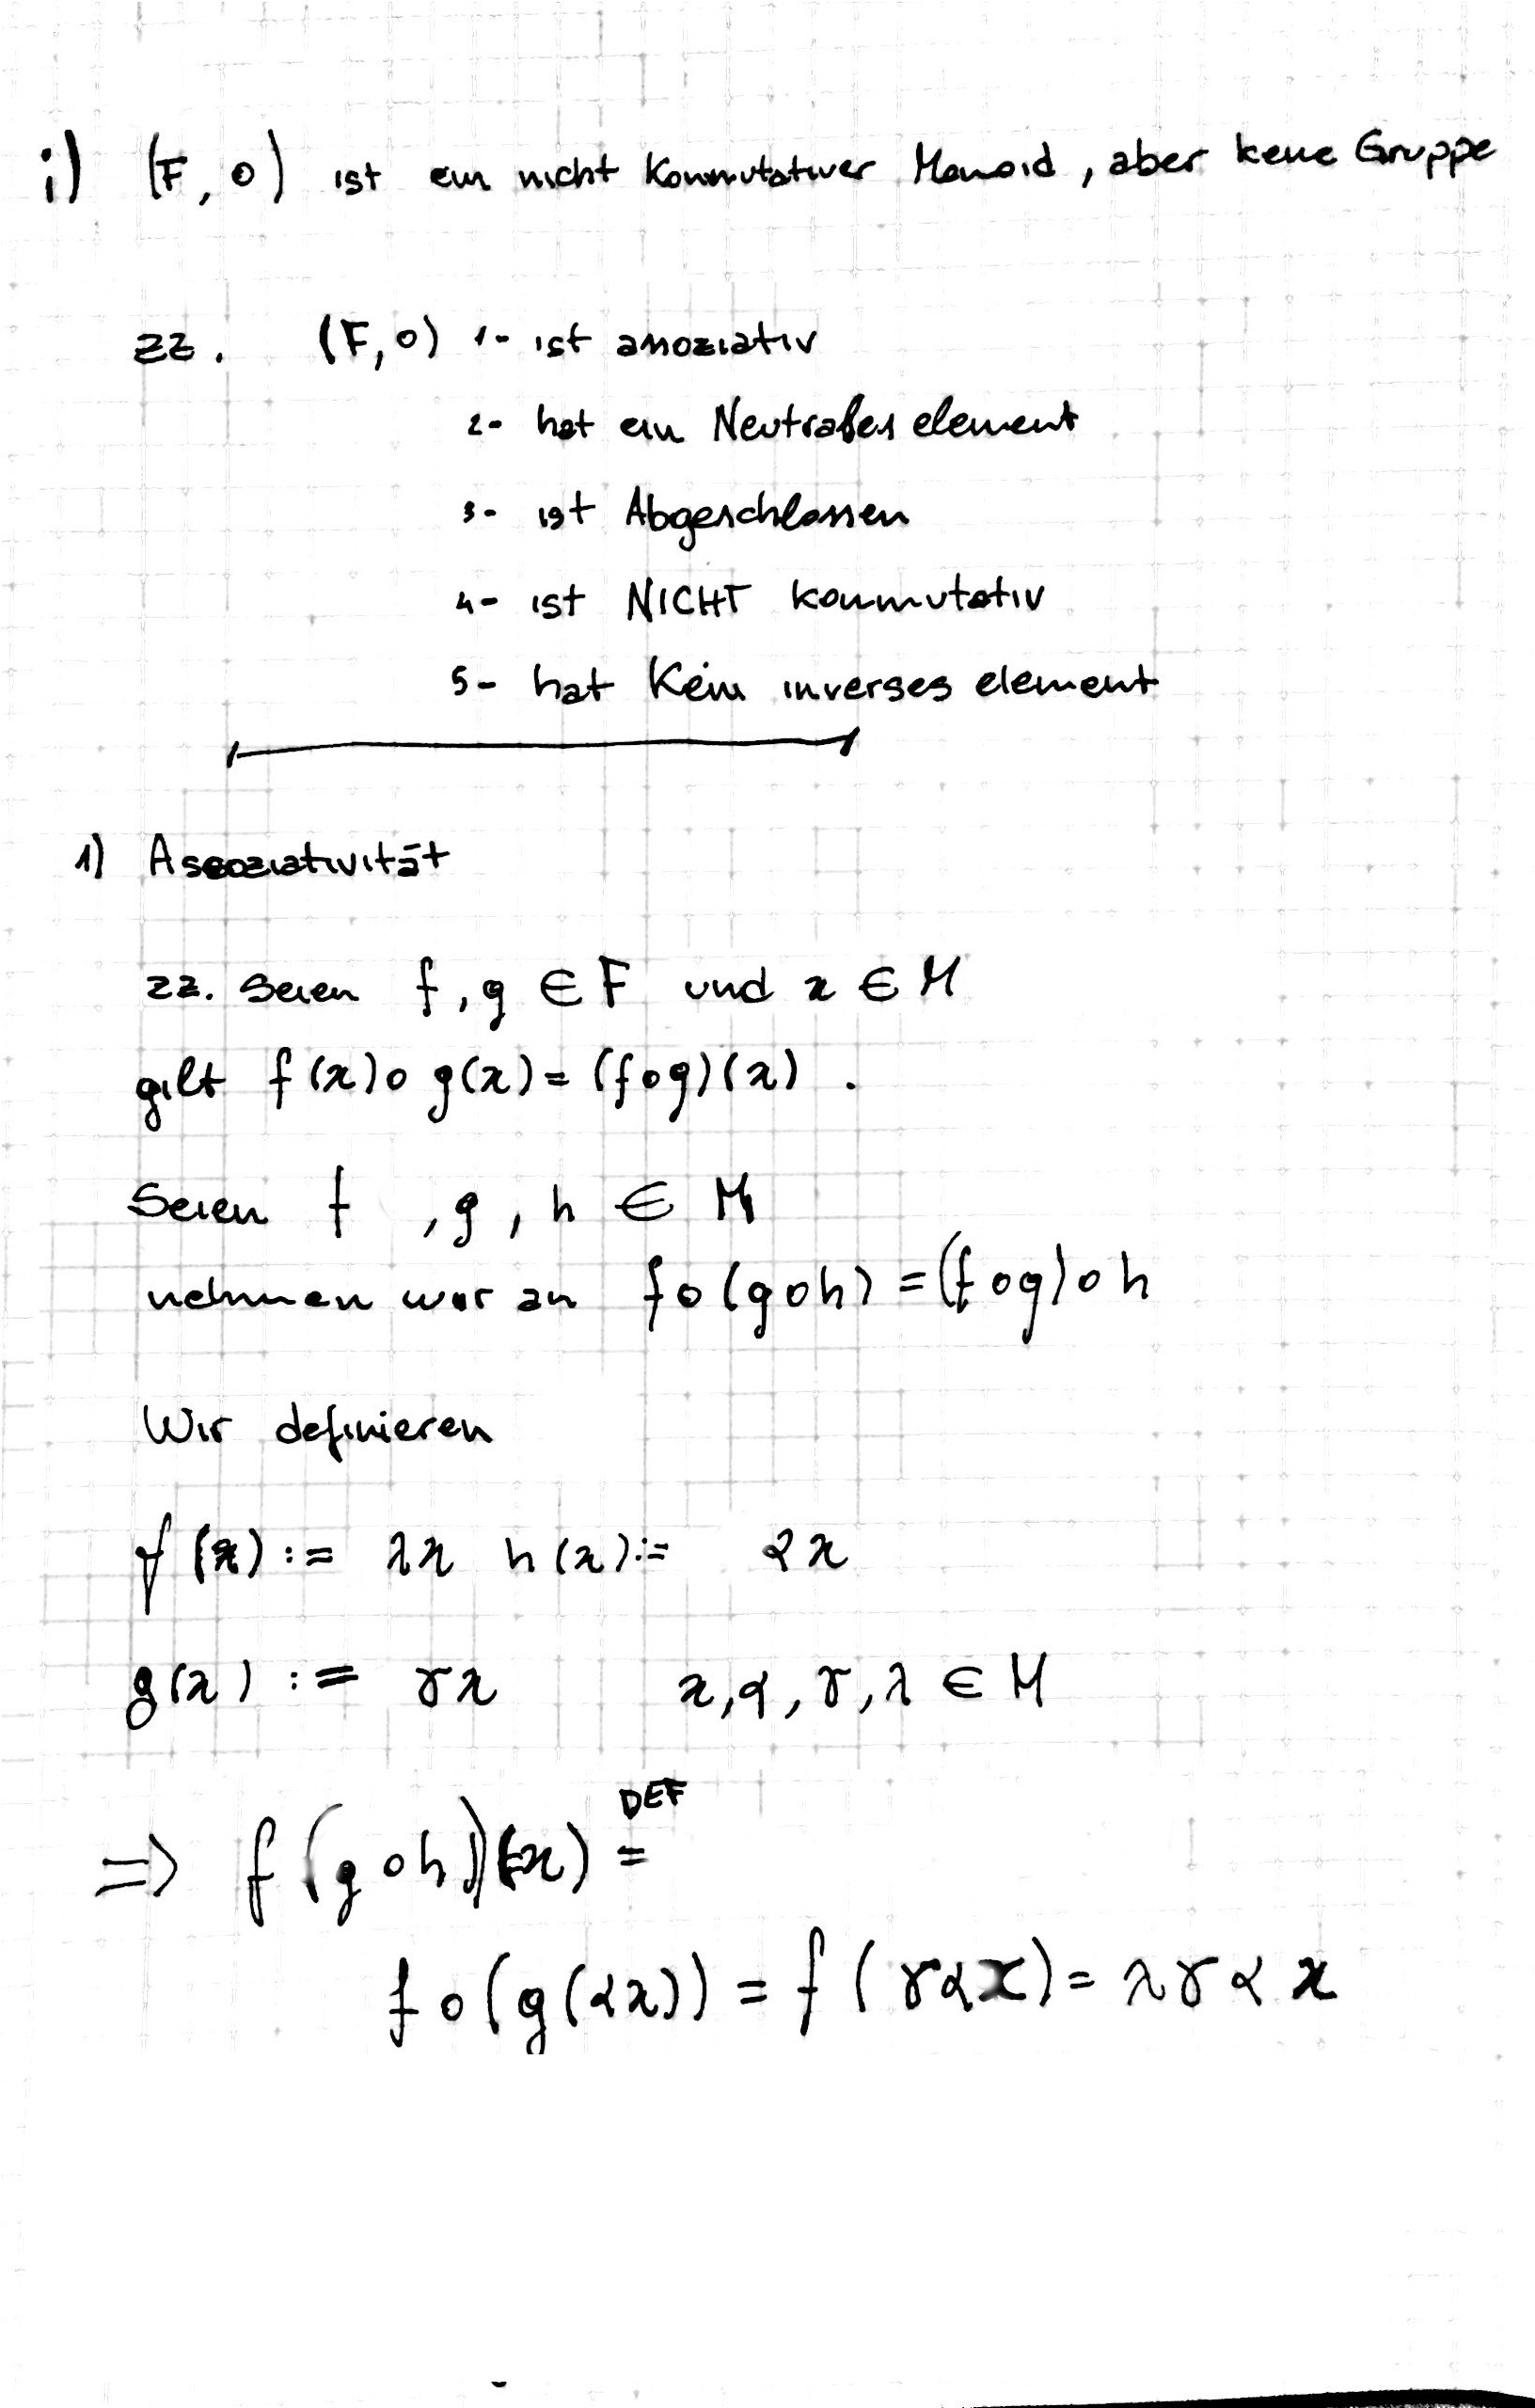
\includegraphics[width=\textwidth]{lat5b_1.jpg}
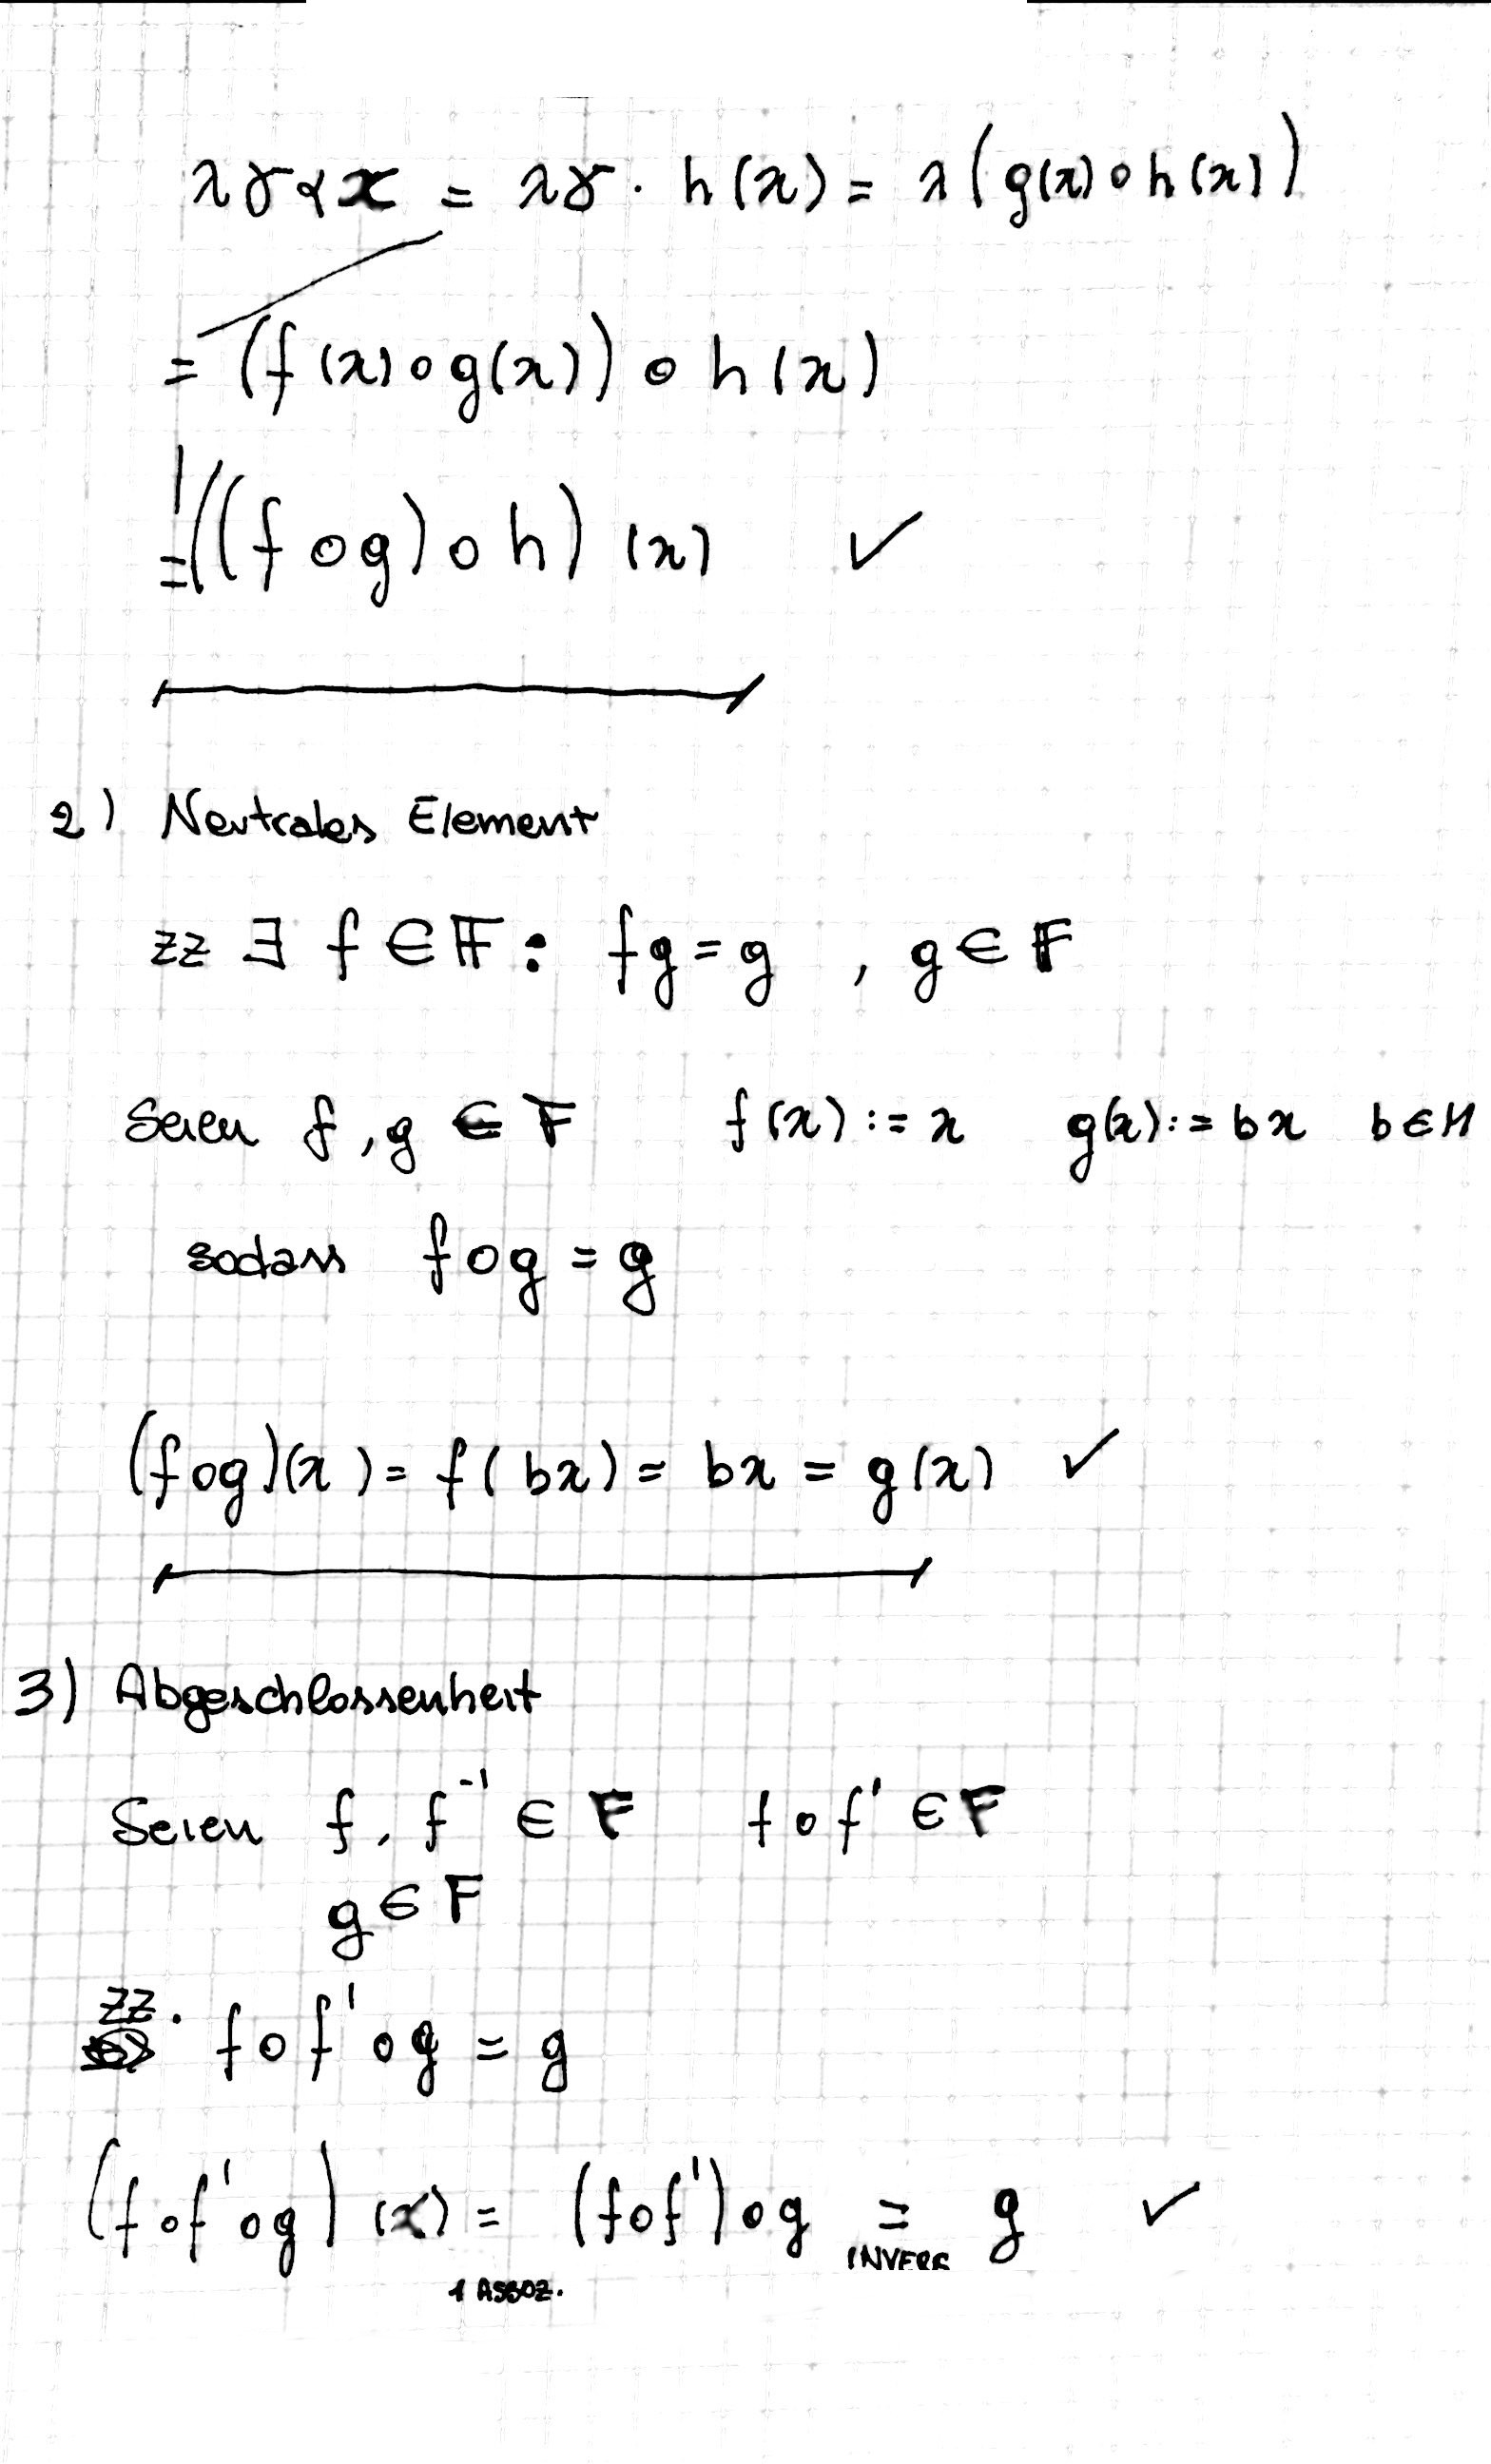
\includegraphics[width=\textwidth]{lat5b_2.jpg}
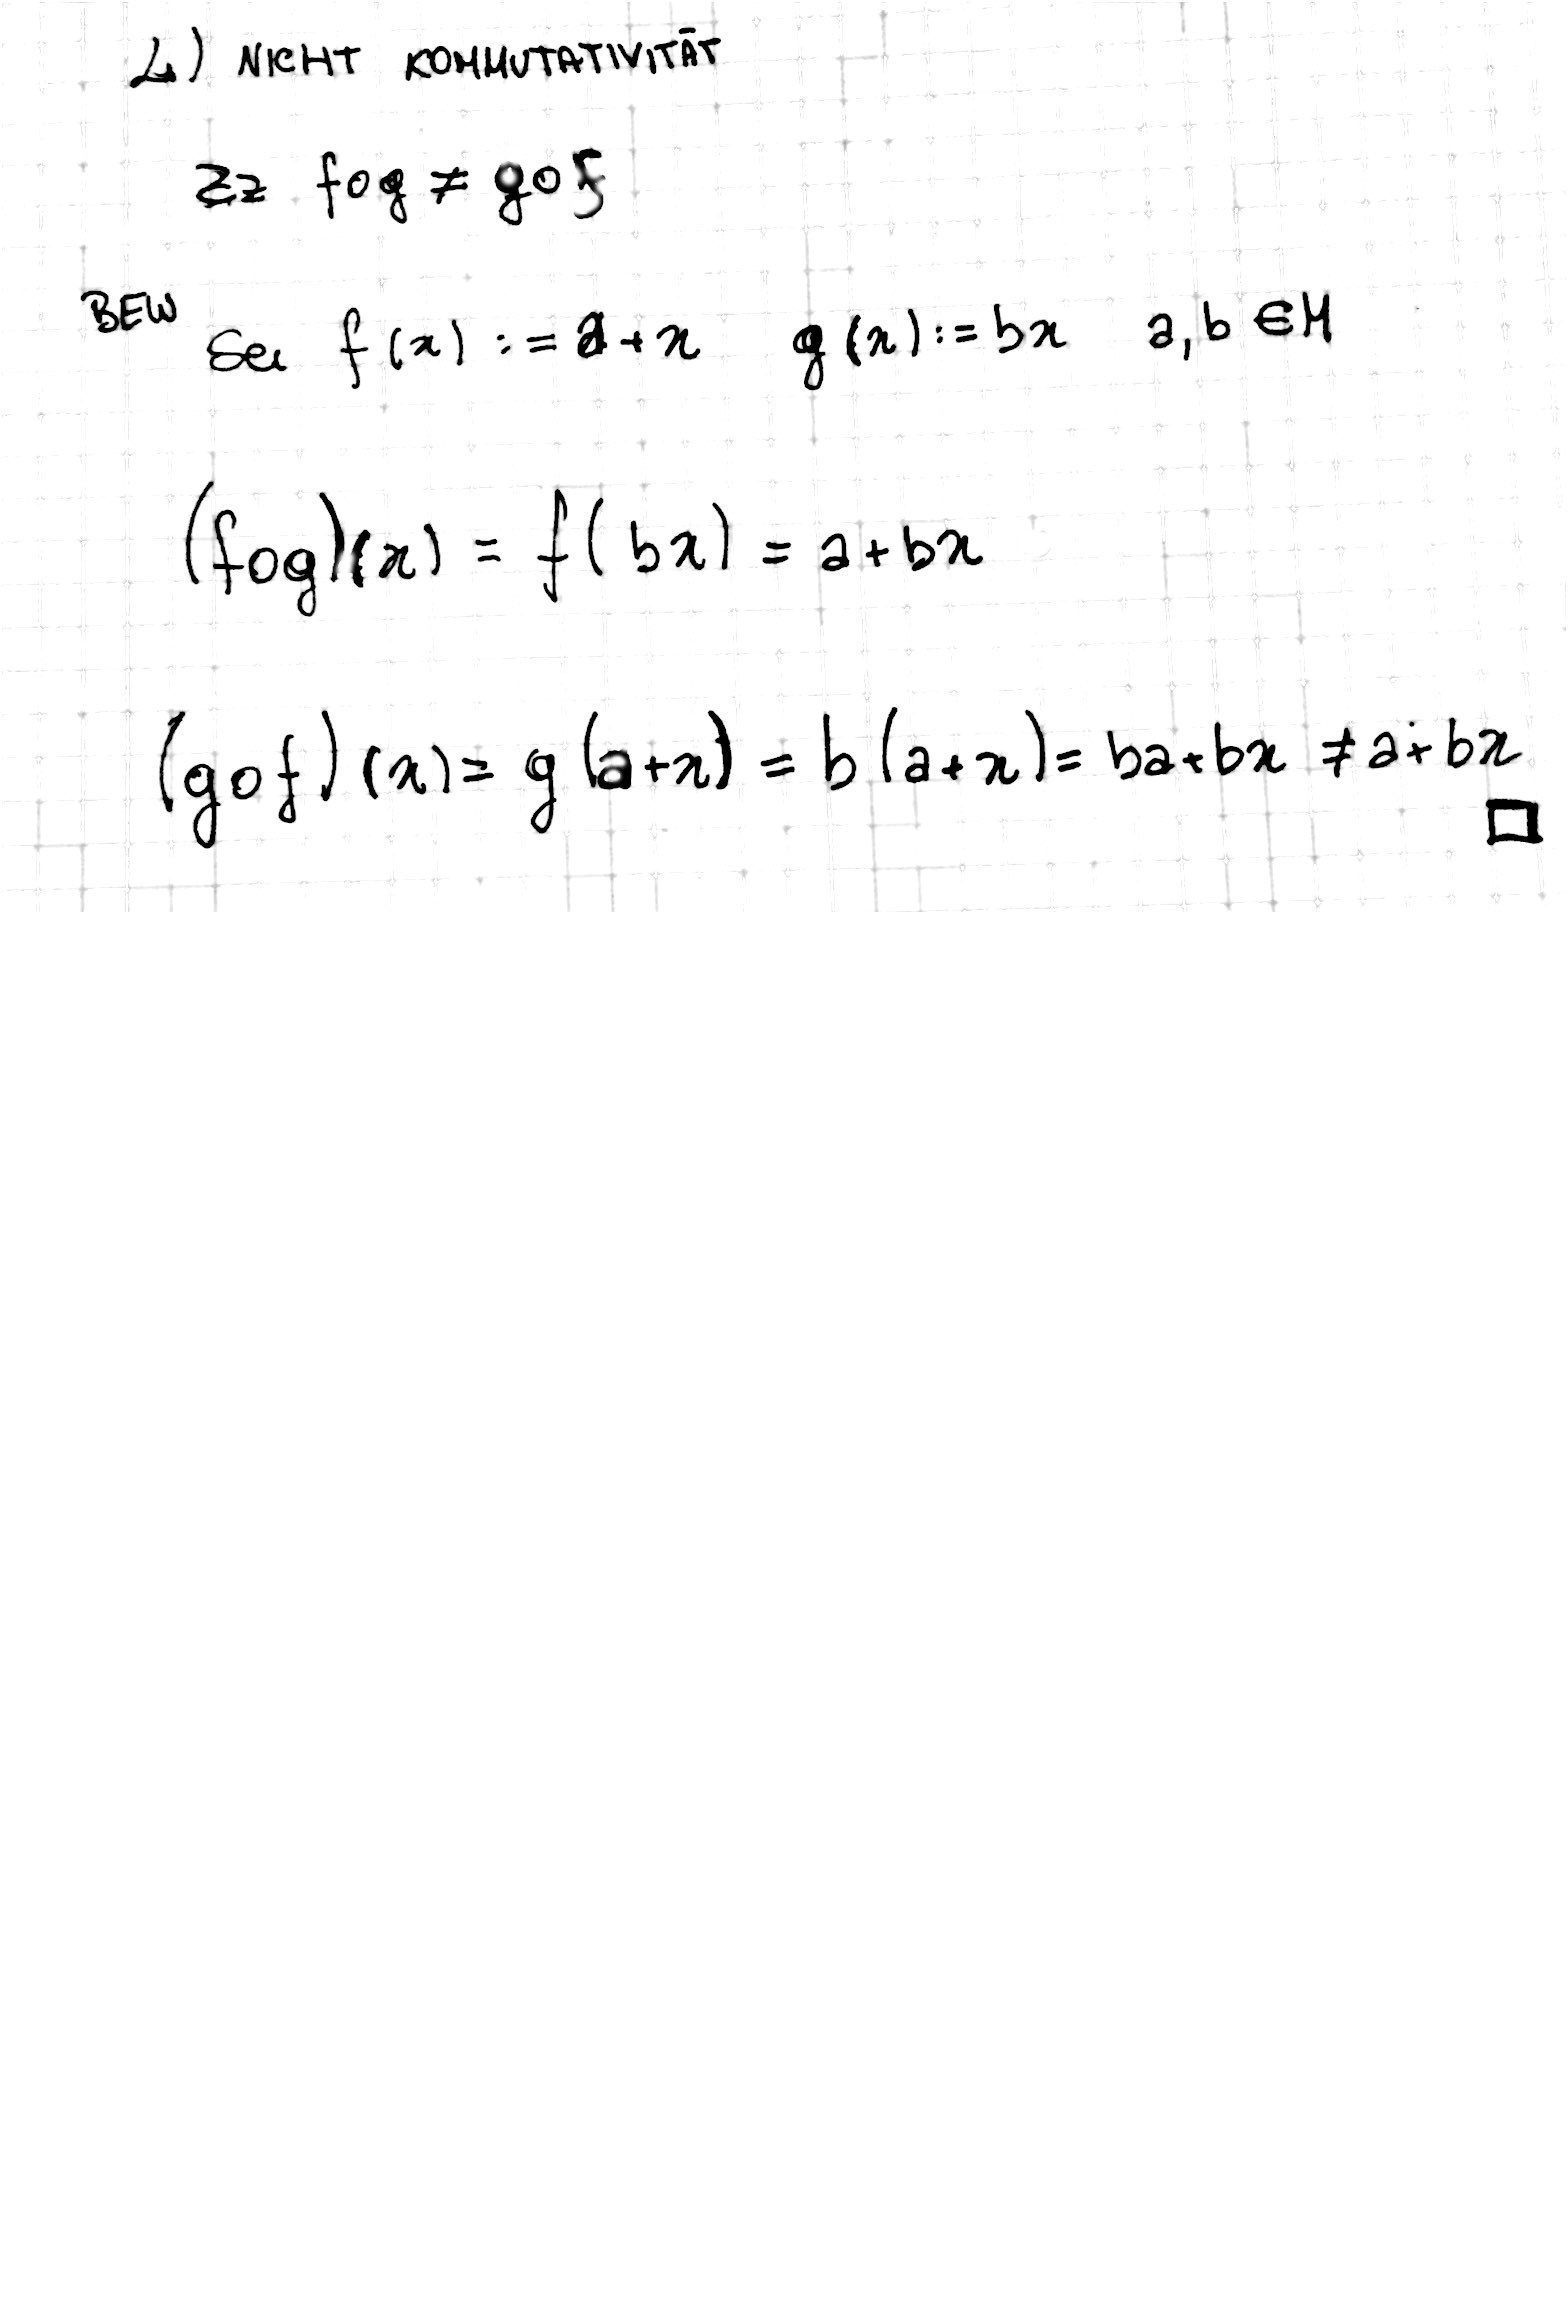
\includegraphics[width=\textwidth]{lat5b_3.jpg}
\subsection{ii}
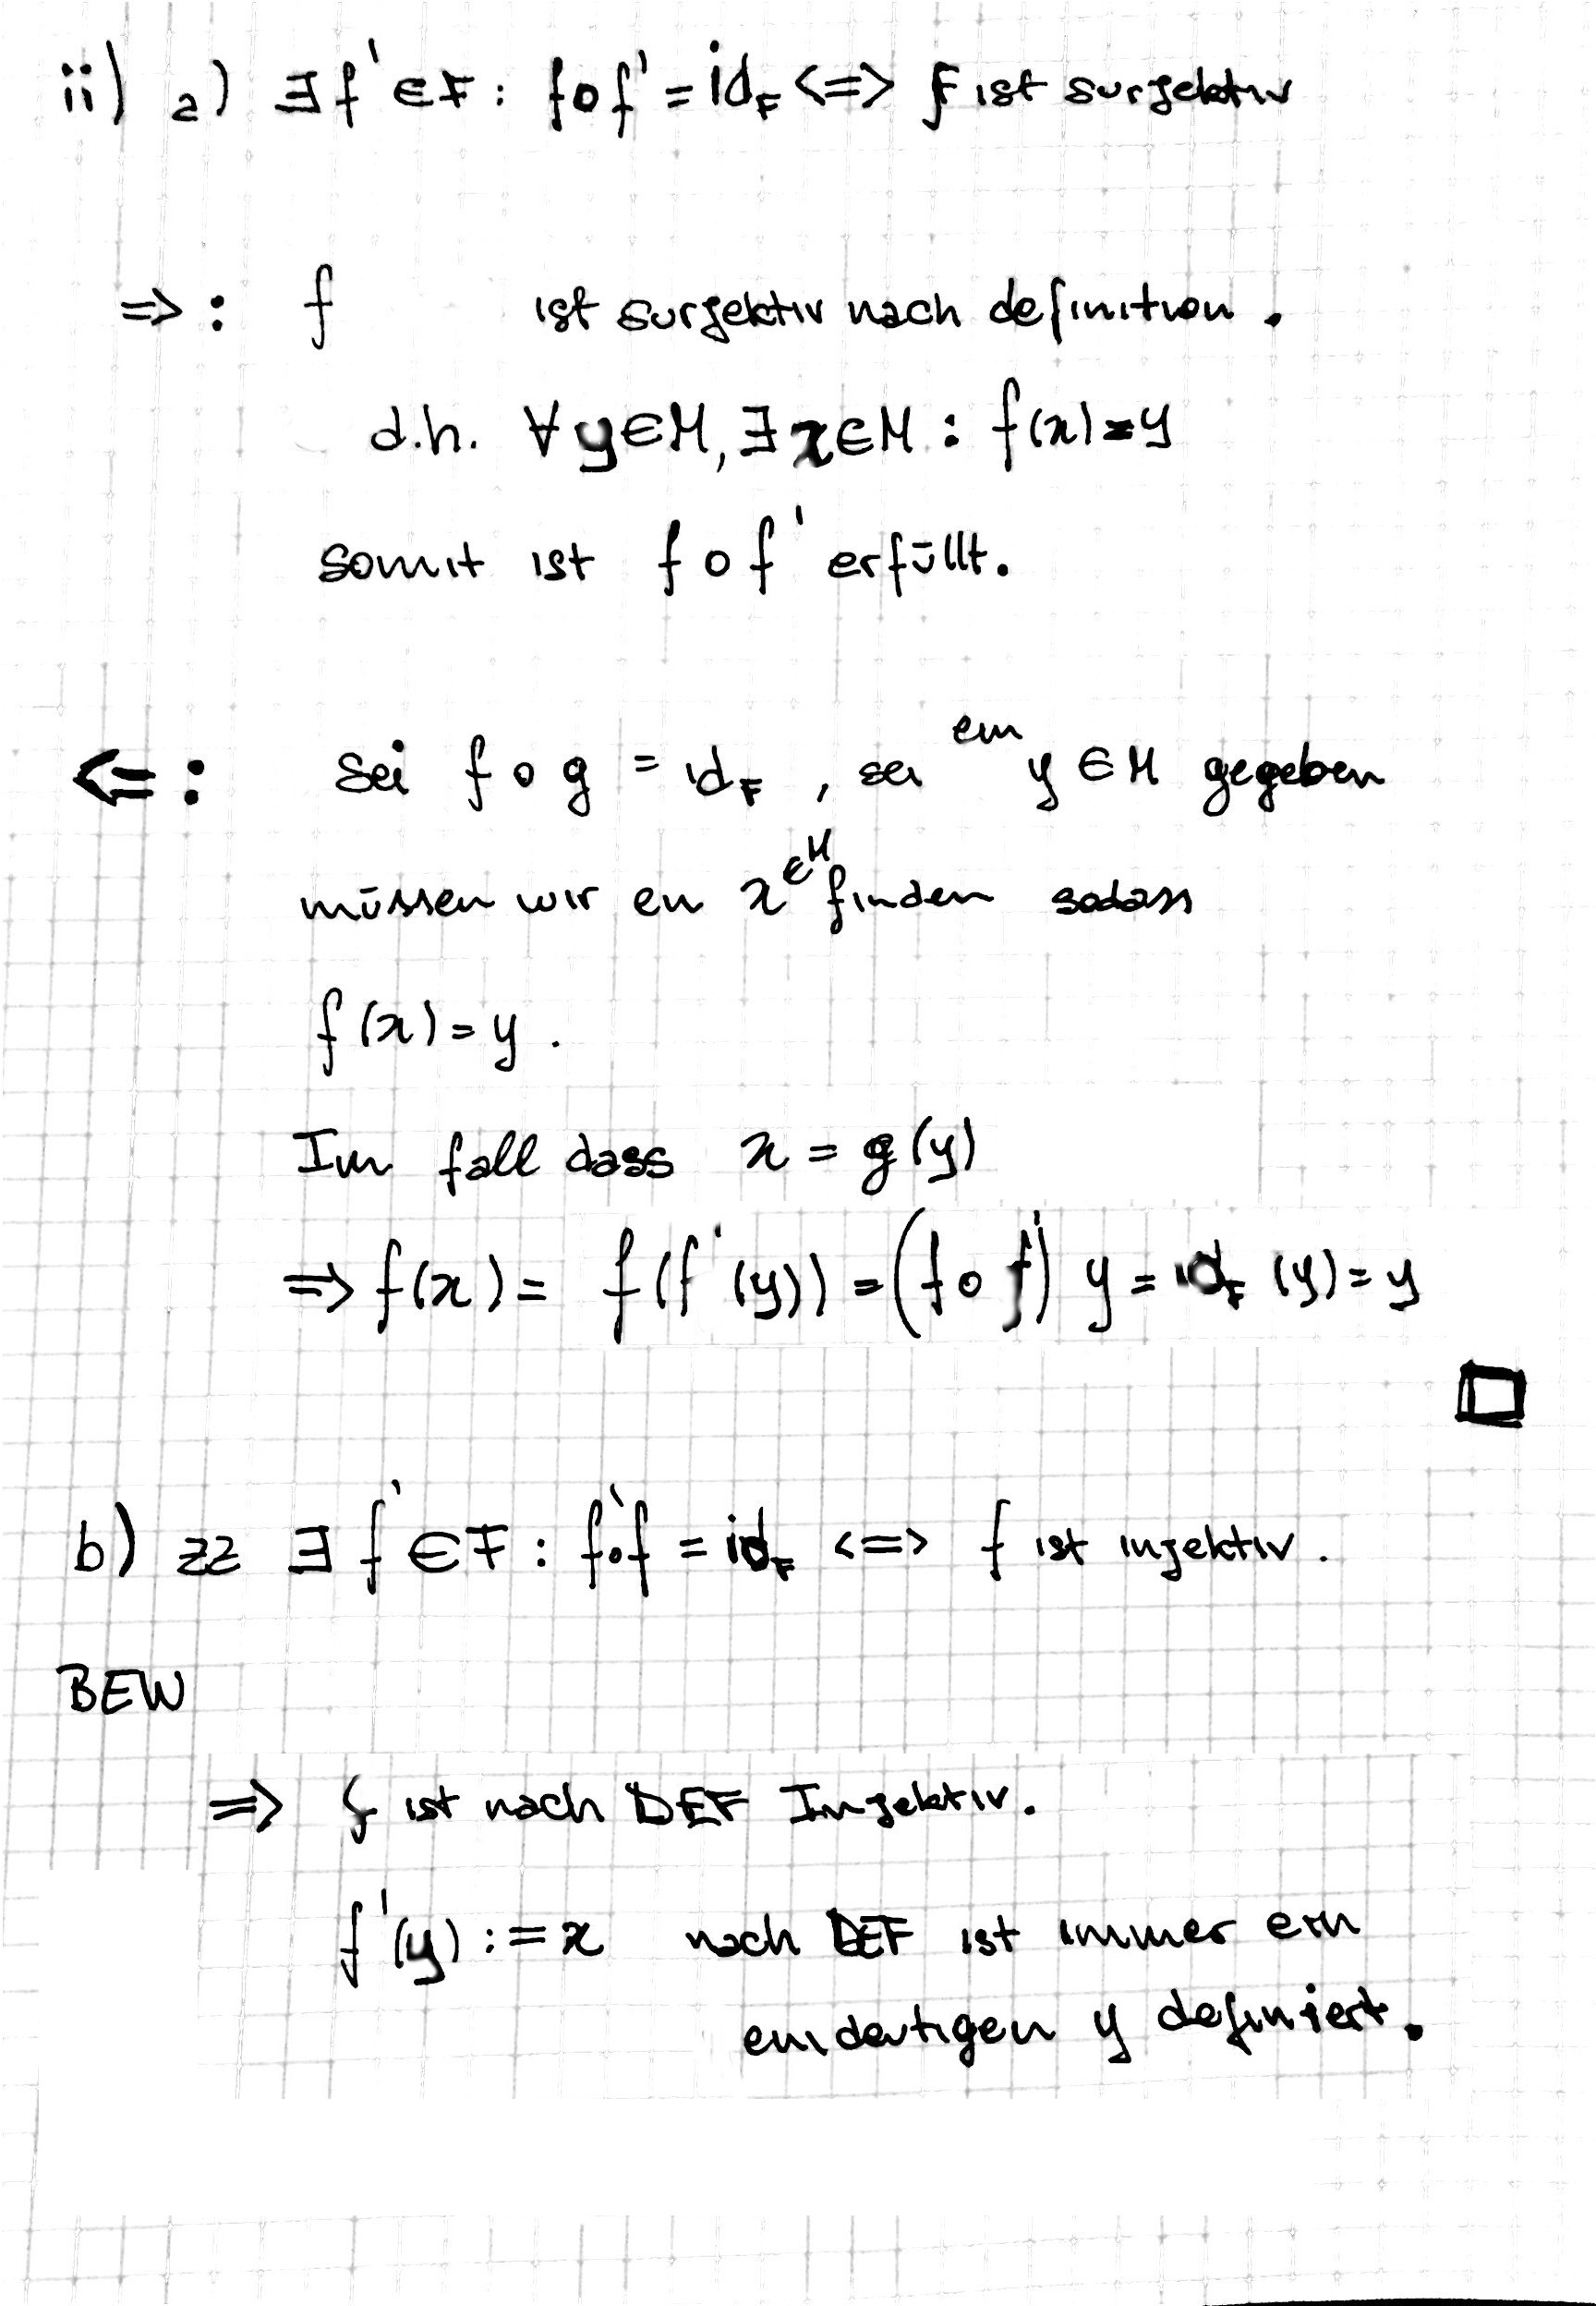
\includegraphics[width=\textwidth]{lat5b_4.jpg}
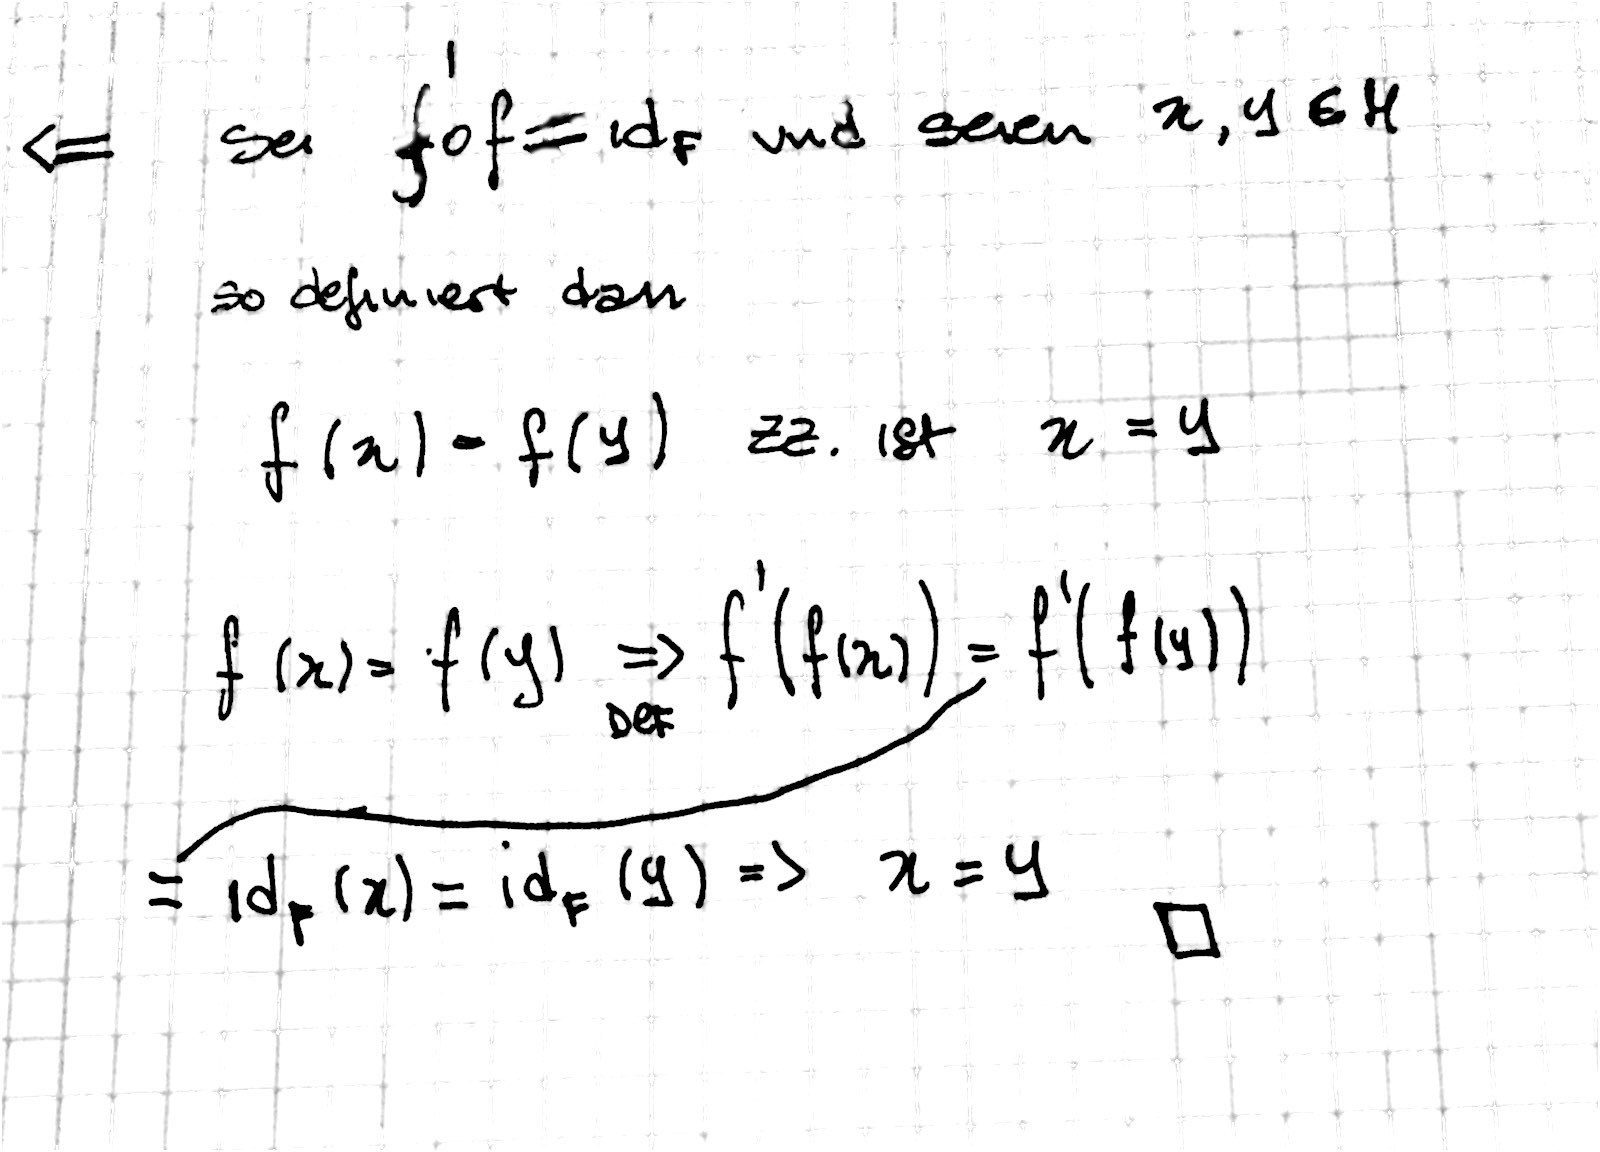
\includegraphics[width=\textwidth]{lat5b_5.jpg}
\subsection{iii}
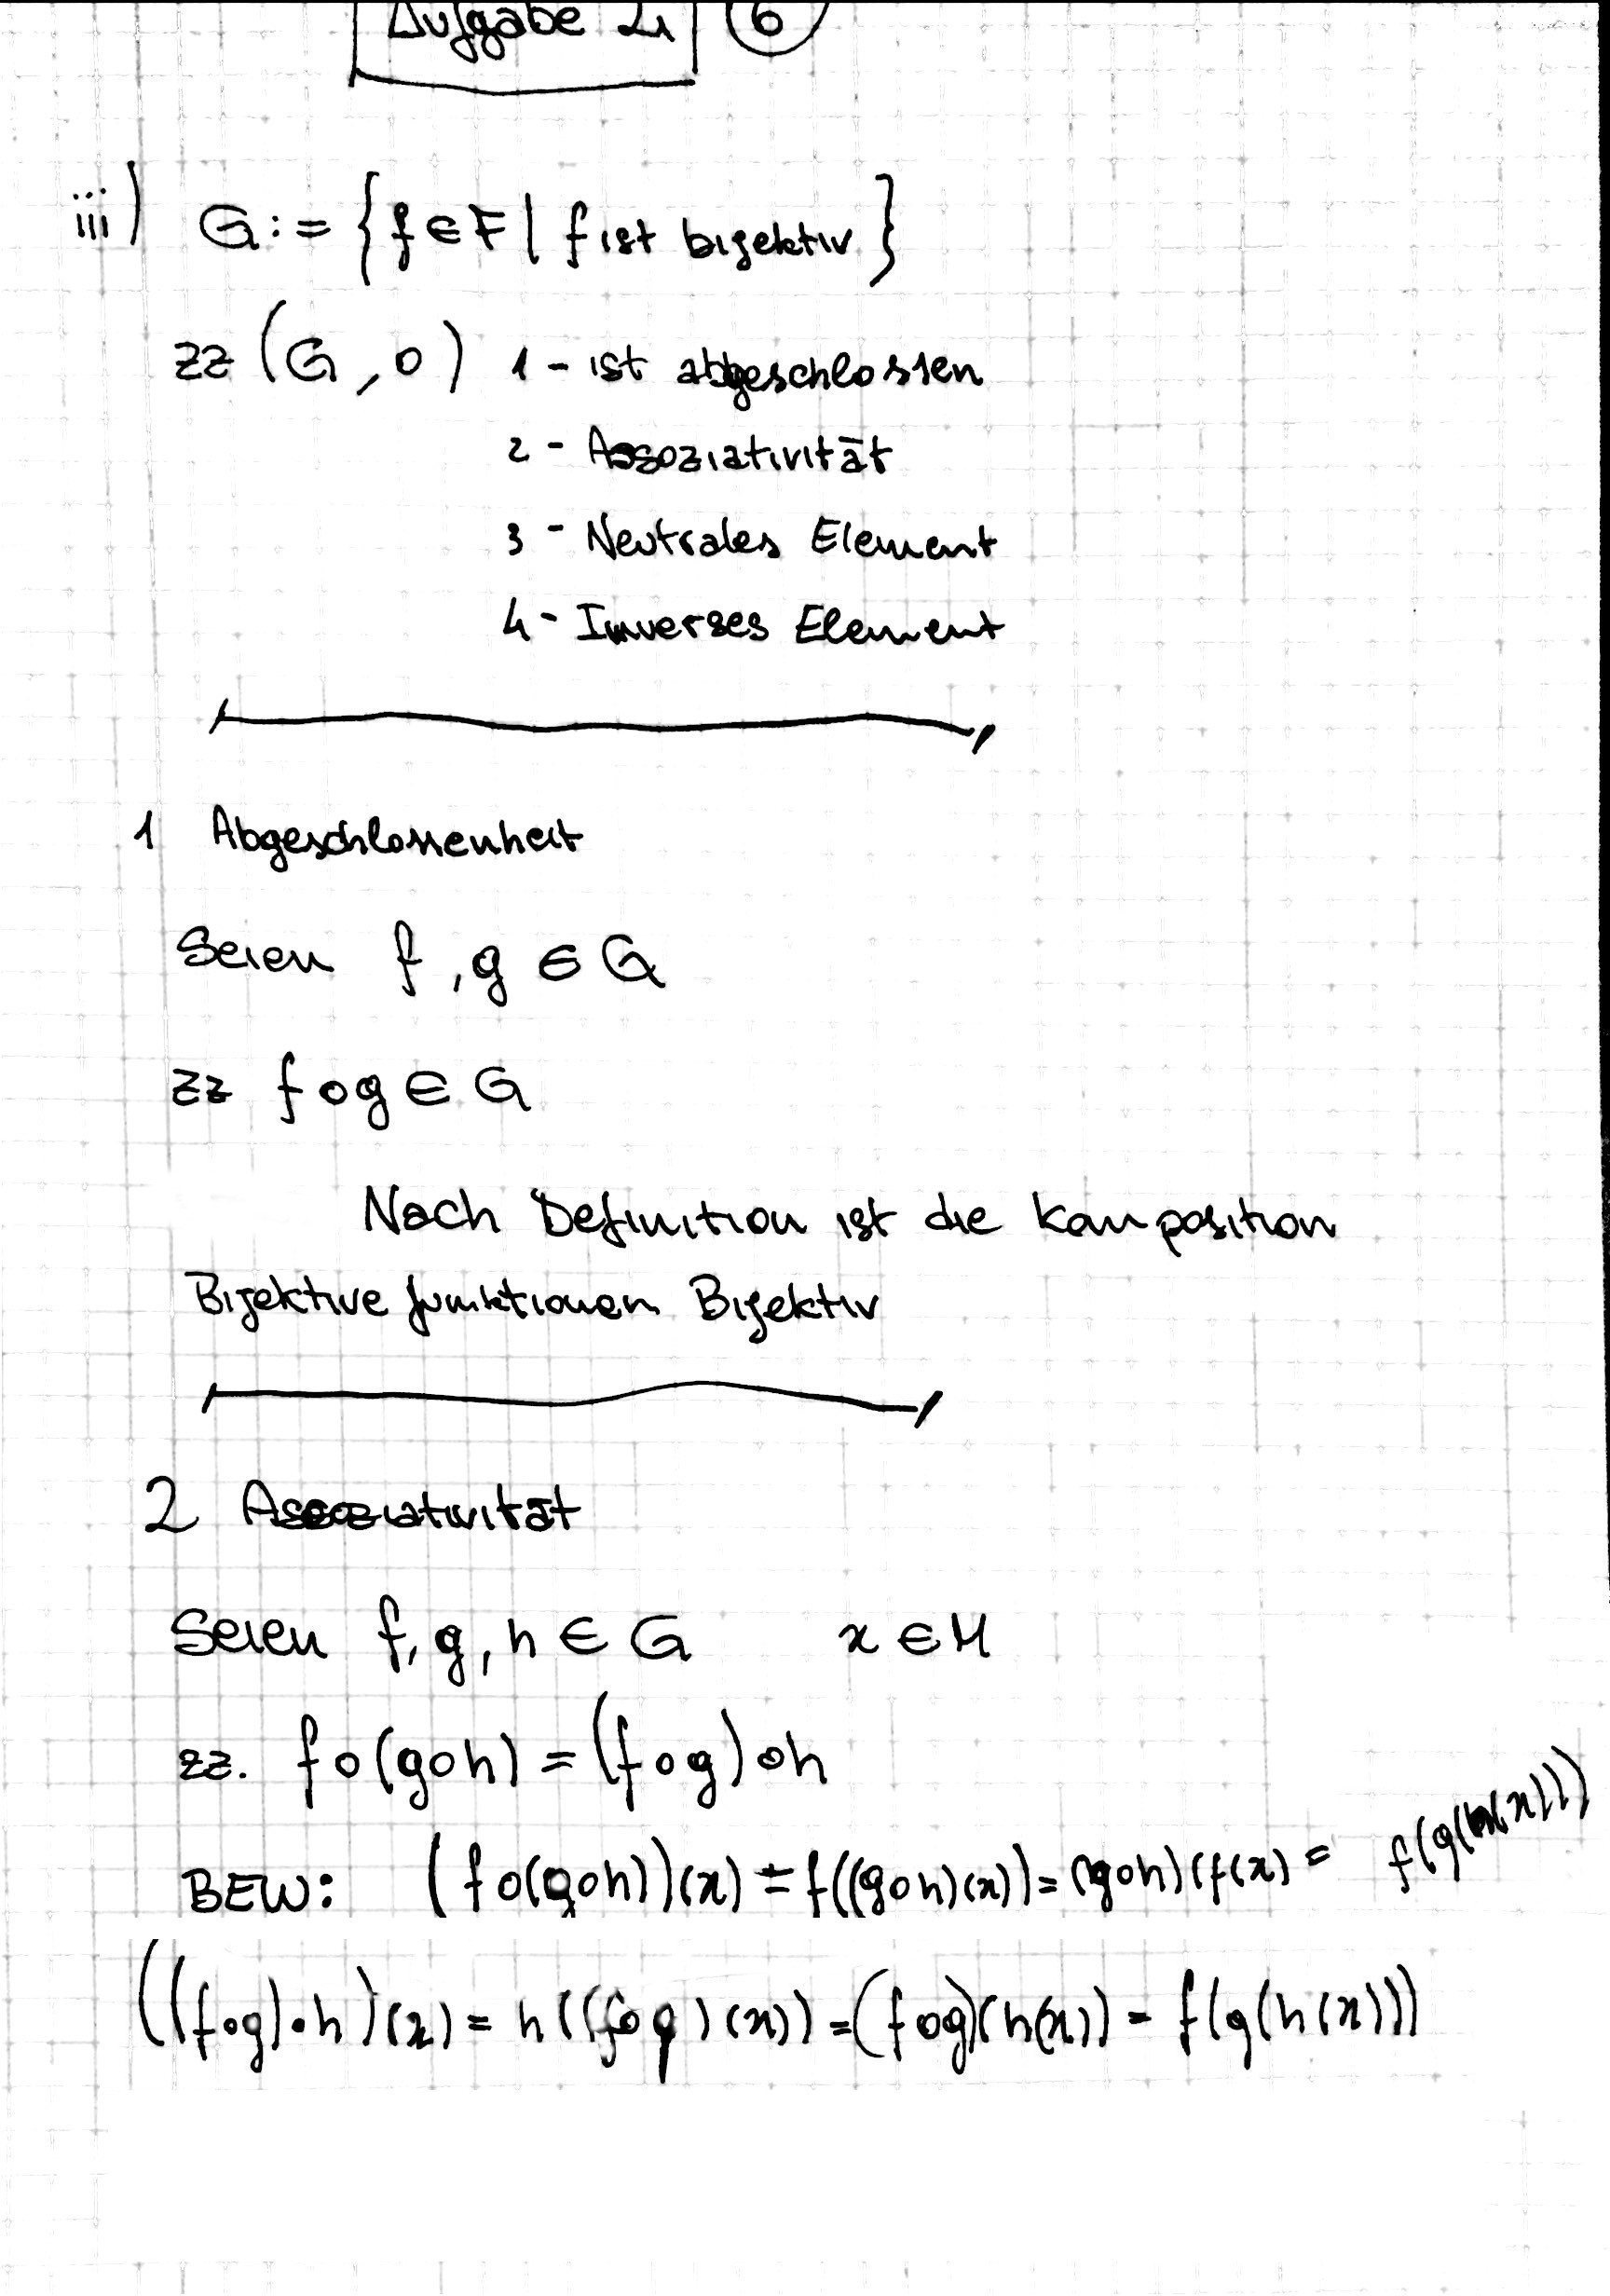
\includegraphics[width=\textwidth]{lat5b_6.jpg}
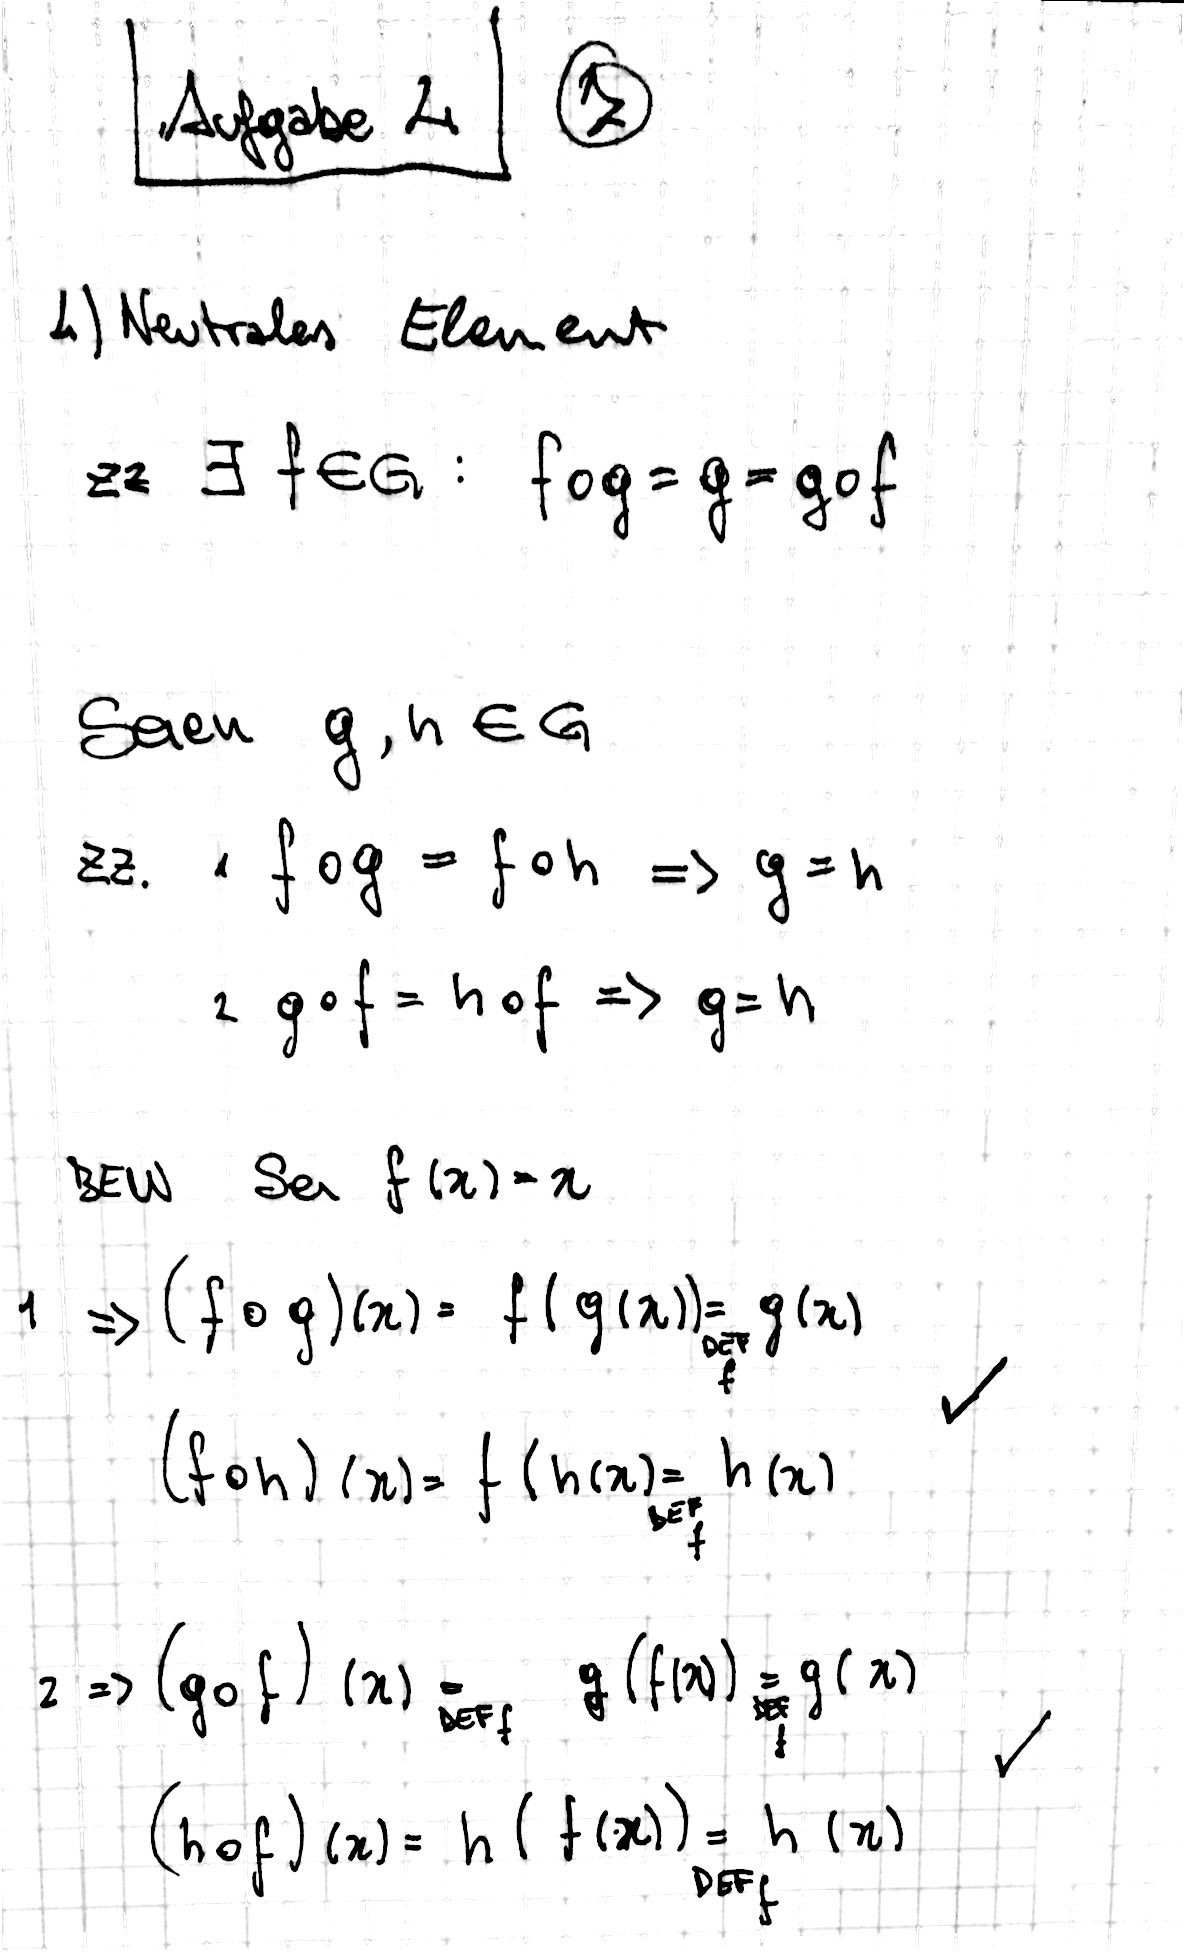
\includegraphics[width=\textwidth]{lat5b_7.jpg}
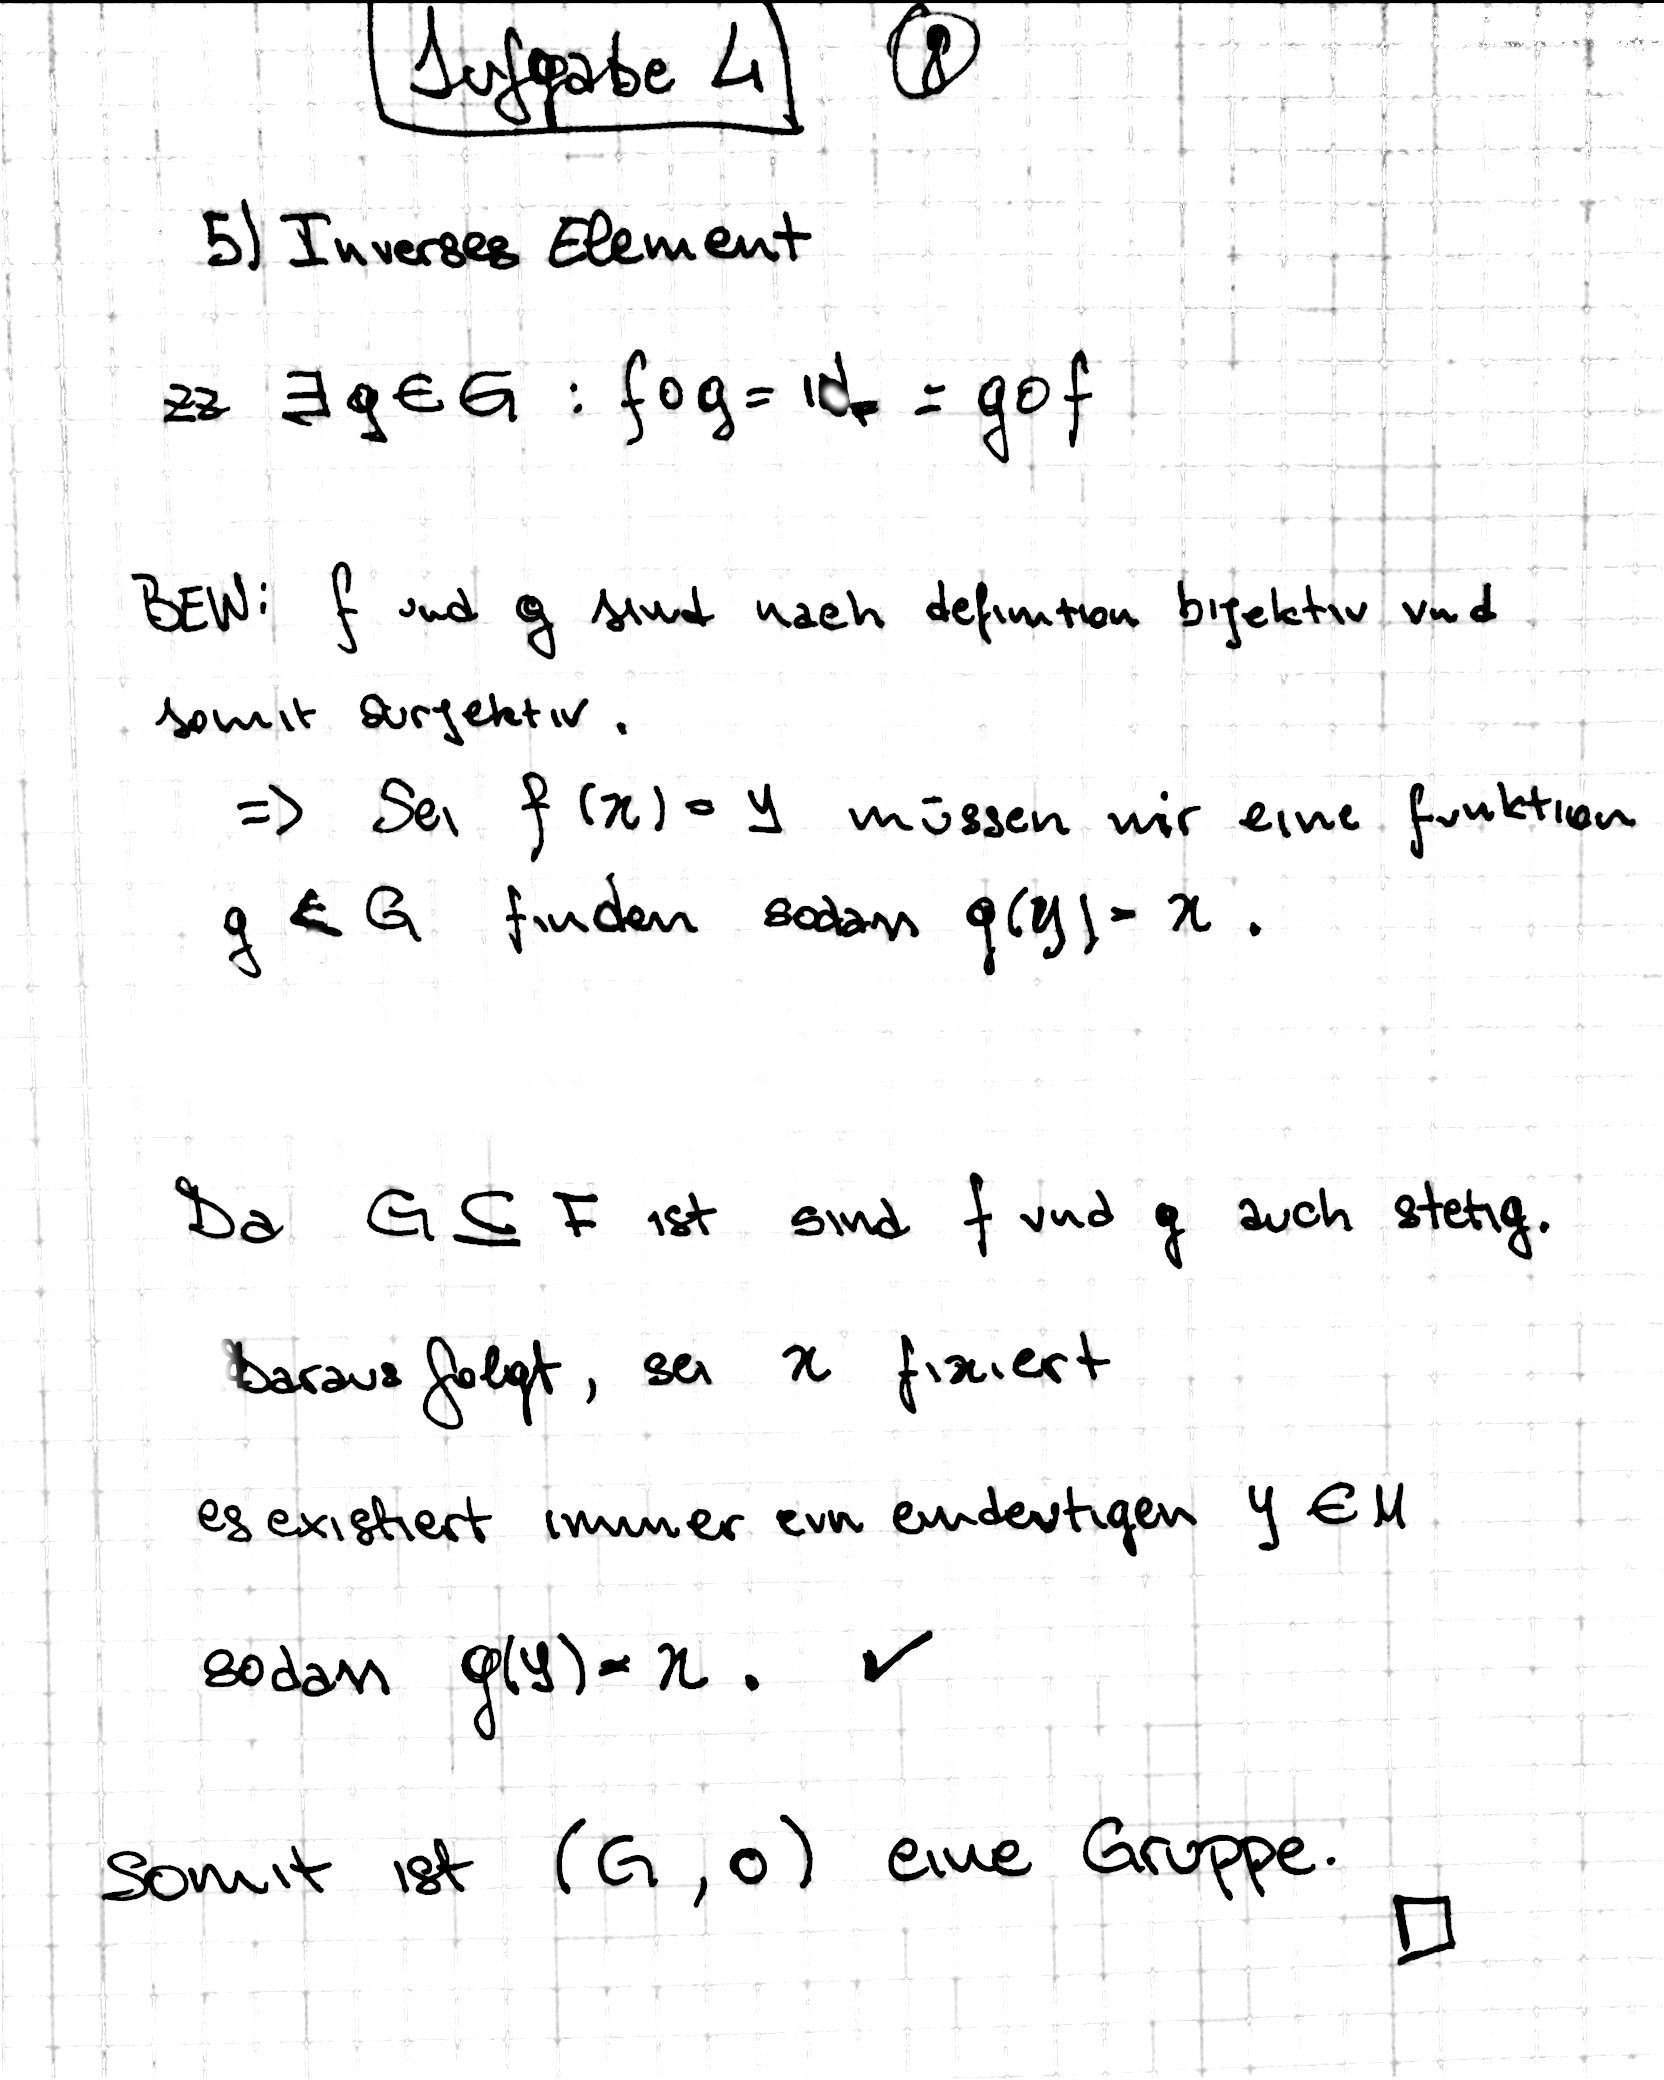
\includegraphics[width=\textwidth]{lat5b_8.jpg}
\subsection{iv}
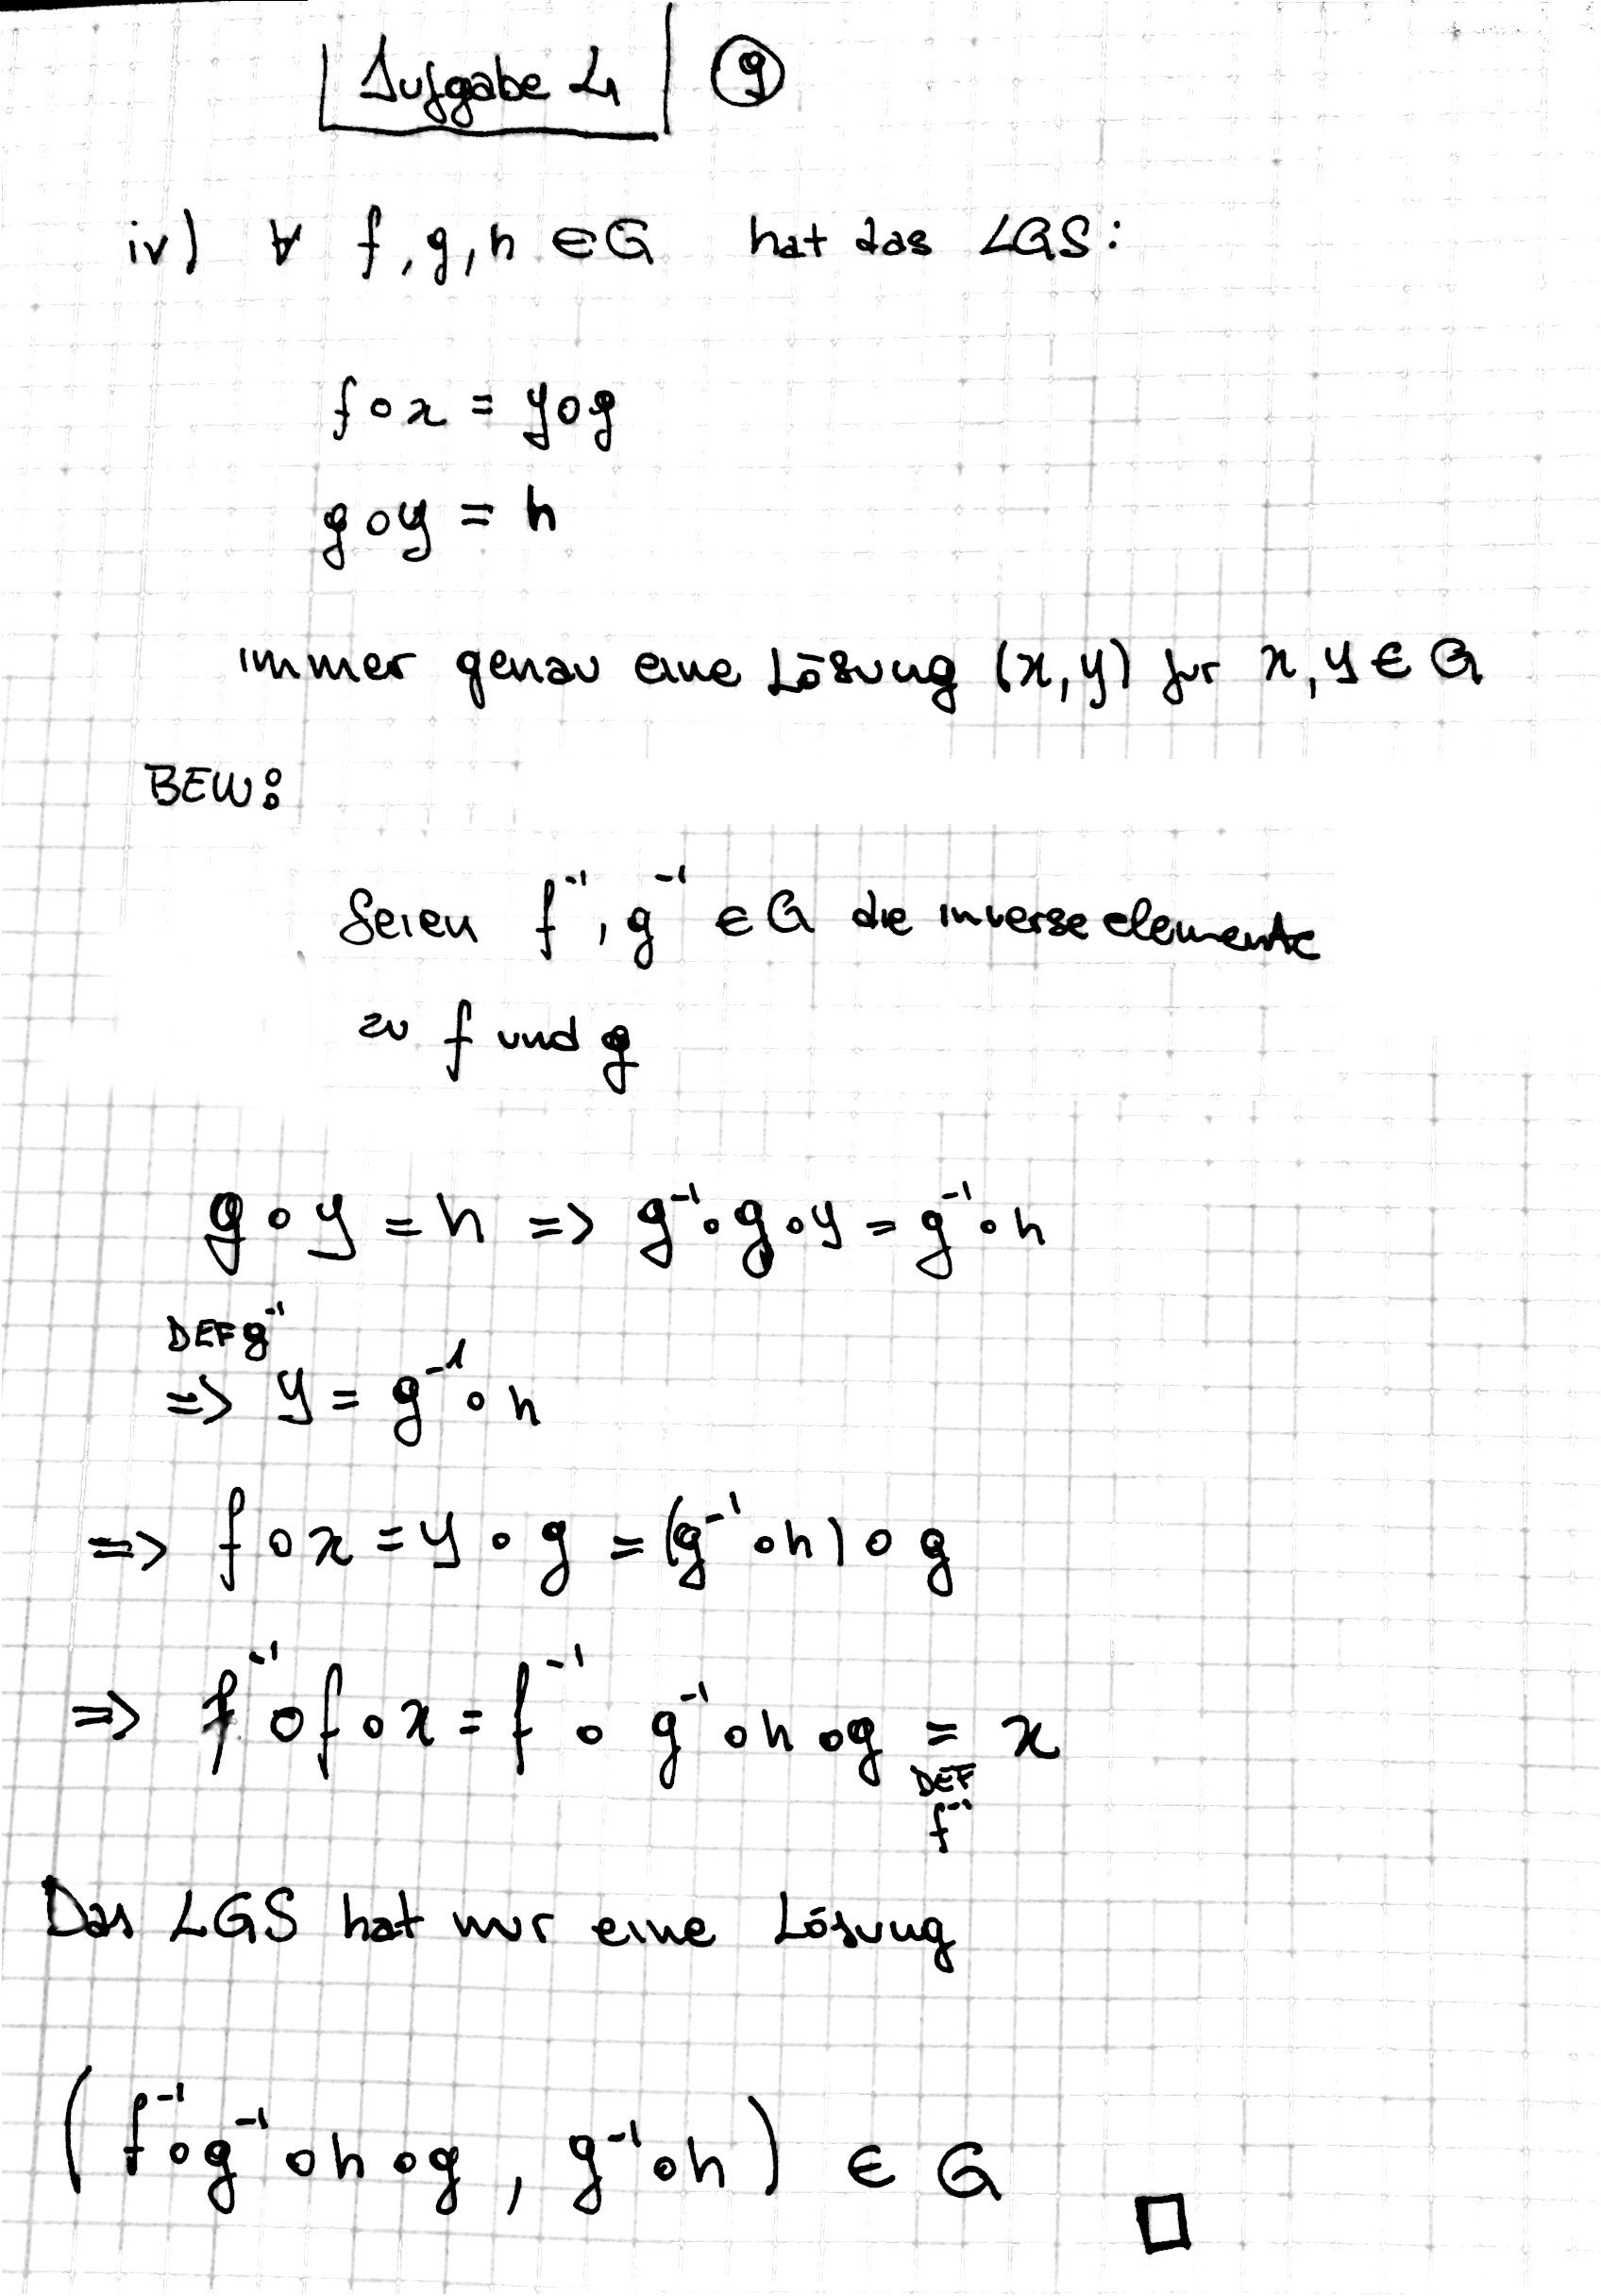
\includegraphics[width=\textwidth]{lat5b_9.jpg} 


\end{document}